
\documentclass[11pt,a4paper]{article}
\usepackage[left=2cm,right=2cm,top=2cm,bottom=3cm]{geometry}
\usepackage{amsmath,amsfonts,amsthm,amssymb,varioref,times, commath}
\usepackage{gensymb}
\usepackage{tikz}
\usepackage{textcomp}
\usepackage{hyperref}
\hypersetup{
 colorlinks=true,
 linkcolor=blue,
 filecolor=magenta, 
urlcolor=cyan,
}
\usepackage{lipsum}
\usepackage{epigraph}
%to resume numbering in a list
\usepackage{enumitem}
%----- arrows 
\usepackage{extarrows}

%    differential equatiosn 
\usepackage{diffcoeff}   %\diff[2]{x}{y}


%%%%%%pour ecrire en français avec les accents
\usepackage[utf8]{inputenc}
\usepackage[T1]{fontenc}
\usepackage{lmodern} % load a font with all the characters
\usepackage{units}
%%%%%%%Image-related packages
\usepackage{wrapfig}
\usepackage{float, graphicx}
\graphicspath{ {./img/} }
\usepackage{subcaption}
\usepackage[export]{adjustbox}

%%%%%%%pour faire des cadres
\usepackage{xcolor}
\usepackage{tcolorbox}
\usepackage{framed}
\usepackage{mdframed}


%%%%%%%chemistry frmulae
\usepackage{chemfig}
\usepackage{chemformula}
\usepackage[version=4]{mhchem}

% -------------- Circuits -------------------
\usepackage[european, straightvoltages]{circuitikz}

% Title & headers
\usepackage[explicit]{titlesec}
% Raised Rule Command:
% Arg 1 (Optional) - How high to raise the rule
% Arg 2 - Thickness of the rule
\newcommand{\raisedrulefill}[2][0ex]{\leaders\hbox{\rule[#1]{1pt}{#2}}\hfill}
\titleformat{\section}{\Large\bfseries}{\thesection. }{0em}{#1\,\raisedrulefill[0.4ex]{1pt}}

% pour ecrire sur +sieurs colonnes
\usepackage{multicol}
\setlength{\columnseprule}{0pt}
\setlength{\columnsep}{60pt}
% Fusion de lignes de tableaux.
\usepackage{multirow}
% Position verticale des lettres dans la ligne de tableau.
\usepackage{array}

% physics -----------------------------------------------------------
\newcommand{\To}{\longrightarrow}
\newcommand{\gpl}{\; g\cdot L^{-1}}
\newcommand{\gpmol}{\; g\cdot mol^{-1}}
\newcommand{\mpl}{\; mol\cdot L^{-1}}
\newcommand{\mps}{\; m\cdot s^{-1}}
\newcommand{\rps}{\; rad\cdot s^{-1}}
\newcommand{\kph}{\; km\cdot h^{-1}}
\newcommand{\mpss}{\; m\cdot s^{-2}}
\newcommand{\Dt}{\Delta t}
\newcommand{\vv}{\vec{v}}
\newcommand{\va}{\vec{a}}
\newcommand{\vp}{\vec{p}}
\newcommand{\vf}{\vec{F}}
\newcommand*{\Vf}[1]{\overrightarrow{F_\ensuremath{{#1}}}}
\newcommand{\es}[1]{\cdot10^{#1}}
\newcommand{\eng}[1]{\textcolor{purple}{(= #1})}
\usepackage{harpoon}
%\newcommand*{\vect}[1]{\overrightharp{\ensuremath{#1}}}
\newcommand*{\Vect}[1]{\overrightarrow{\ensuremath{#1}}}
\newcommand{\pfd}[1]{\sum \vec{F}_{ext_{#1}} &= \od{\vp_{#1}}{t} = m\cdot\va_{#1}}
\newcommand{\C}{\degree C}
\newcommand{\Delt}{\Delta t}

% --- Circuits ------------
\newcommand{\bipole}[1]{
\begin{circuitikz} \draw
(0,0) to[ #1 ] (2,0); 
\end{circuitikz} {\hspace{5mm}}}

% Chimie ---------------------------------
\newcommand{\oxo}{\ce{H3O+}_{(aq)}}
\newcommand{\eau}{\ce{H2O}_{(\ell)}}
\newcommand{\OH}{\ce{HO-}_{(aq)}}
\newcommand{\AH}{\ce{AH}_{(aq)}}
\newcommand{\A}{\ce{A-}_{(aq)}}
\newcommand{\MnO}{\ce{MnO_4^{-}}}
\newcommand{\conc}[1]{\left[{#1}\right]}
\newcommand{\couple}[2]{\ce{#1/#2}}


% Environnements ------------------------
\newcounter{exo}
\newenvironment{exo}[1][]
{\refstepcounter{exo} \begin{shaded}\noindent $\triangleright \quad$\textbf{Exercice~\theexo. #1} } { \end{shaded}}
\newenvironment{eg}
{\begin{shaded} \textbf{Exemple:} } { \end{shaded}}

\newenvironment{defn}[1]
{\begin{leftbar}\noindent \textbf{Définition :\textit{ \quad #1}} } { \end{leftbar}}

%\newenvironment{rmrq}
%{\begin{shaded} \textbf{Remarque.\quad } \itshape } { \end{shaded}}
\newenvironment{rmrq}
{\begin{mdframed}[backgroundcolor=blue!10, linewidth=0pt] \textbf{Remarque.\quad } \itshape } { \end{mdframed}}

\newenvironment{python}
{\begin{shaded} \textbf{A faire en PYTHON}\\ \itshape } { \end{shaded}}

% Shading colour -----------------------------
\definecolor{shadecolor}{gray}{0.9}

\date{}
\author{}

\renewcommand*\contentsname{Résumé}









% Title & headers 
\usepackage{fancyhdr}
\pagestyle{fancy}
\fancyhf{}
\lhead{SciPhy : Terminale spé}
\rhead{$\chi $ - 1 : Mesures \& Dosages}
\chead{2020-28}
\rfoot{Page \thepage}
\lfoot{\textcopyright\; S Zayyani}
\renewcommand{\footrulewidth}{0.1pt}% default is 0pt

\title{\large Chimie - Chapitre 1 \\ \LARGE Mesure physiques \& chimiques}
\date{}
\author{}

\setlength{\parindent}{0mm}
\setlength{\parskip}{2mm}

%%%%%%%%%%% For wrapfigure 
\setlength{\intextsep}{3pt}%
\setlength{\columnsep}{3pt}%



\begin{document}
\maketitle
\vspace{-1cm}
\begin{tcolorbox}[title=Notions de la classe de première à rappeler]
Dosages ; réaction rédox ; avancement de réaction ; tableau d'avancement ; Loi de Beer-Lambert 
%\tcblower
\end{tcolorbox}
\tableofcontents

\section{Spectroscopie}
\begin{defn}{Spectroscopie}
\begin{itemize}
    \item la spectroscopie est une technique d'analyse de la matière basée sur l'étude de ses interactions avec des radiations électromagnétiques. 
    \item La spectroscopie, ou spectrométrie, est l'étude expérimentale du spectre \eng{spectrum} d'un phénomène physique. 
    \item il existe de différentes formes de spectroscopie: UV-visible, IR, RMN, micro-onde, etc. 
\end{itemize}
\end{defn}



\subsection{Spectrophotométrie : lumière UV - visible}
Vous avez déjà vu les principes de la spectrophotométrie en première, mais nous allons faire une petite révision quand-même. 

\begin{defn}{Absorbance}
\begin{itemize}
    \item L'\textbf{absorbance} est la grandeur physique qui caractérise l'absorption par une substance d'une radiation lumineuse de longueur d'onde donnée. 
    \item Notée $A$, l'absorbance est une grandeur sans unité. Un corps qui est totalement transparent aura donc déjà une absorbance de $0$; et l’absorbance d’un corps totalement opaque, à une radiation lumineuse, est théoriquement infinie. 
    \item L'inverse de l'absorbance s'appelle la \textbf{transmittance}, noté $T$. La relation entre l'absorbance et la transmittance est donnée par $ A = -\log(\frac{1}{T})$:  Toutes les deux sont exprimées en pourcentage. 
\end{itemize}
\end{defn}

\begin{defn}{Spectrophotométrie}
\begin{itemize}
    \item La spectrophotométrie est une méthode analytique quantitative qui consiste à mesurer l'absorbance ou la densité optique d'une substance chimique donnée, généralement en solution. Plus l'échantillon est concentré, plus il absorbe la lumière dans les limites de proportionnalité énoncées par la loi de Beer-Lambert (cf. ci-dessous).
    \item La densité optique des échantillons est déterminée par un spectrophotomètre préalablement étalonné sur la longueur d'onde d'absorption de la substance à étudier.
\end{itemize}
\end{defn}

Finalement, la relation qui nous permet d'exploiter les variation de l'absorbance afin de déterminer les variations de la concentration : Loi de Beer-Lambert. 

\begin{defn}{Loi de Beer-Lambert}
\begin{itemize}
    \item 	la relation entre l'absorbance d'une radiation d'une longueur d'onde donnée et la concentration molaire du soluté c de la solution est donnée par la loi de Beer-Lambert:
    \[
    A = \epsilon\cdot\ell\cdot c \quad \text{  où  }\quad 
    \begin{cases}
    \epsilon \rightarrow \text{}(L\cdot cm^{-1}\cdot mol^{-1}) \\
    \ell \rightarrow \text{épaisseur de la solution }(cm)\\
    c \rightarrow \text{concentration }(\mpl ) \\
    \end{cases}
    \]
    \item $\epsilon$ epsilon s'appelle le \textbf{coefficient d'absorption molaire}. Il dépend de l'espèce, du solvant, de la température, et de la longueur d'onde
    \item Si la solution contient plusieurs espèces qui absorbent à la même longueur d’onde, l’absorbance de la solution est égale à la somme des absorbance liées à chaque espèce : $A=\epsilon_1\cdot\ell\cdot c_1 + \epsilon_2\cdot\ell\cdot c_2$
\end{itemize}
\end{defn}

\subsection{Infrarouge IR}

La spectroscopie IR est l’étude de l’absorption des ondes EM comprises supérieure à $800\; nm$, par des composés organiques. 

En résumé, le rayonnement IR est moins énergétique que les rayonnements UV ou lumineux. Mais l’énergie apportée par ces rayonnements IR est suffisante pour mettre les liaisons chimiques entre les différents atomes d’un composé chimique « en vibration ». 

La longueur d’onde du rayonnement IR absorbé dépend de la nature de la liaison : comme on verra une liaison $\ce{C-H}$ n’a pas besoin de la même énergie pour se mettre en mouvement qu’une liaison $\ce{C=O}$, par exemple.  

Grâce à un \textit{spectromètre infrarouge}, nous pouvons obtenir le spectre IR d’un composé organique. Ce dernier est le tracé de la transmittance $T$ (et donc l’absorption selon $A = -\log(\frac{1}{T})$) en $\%$ en fonction de la longueur d’onde du rayonnement IR. En observant où se situent les bandes d'absorption les plus importantes (en fonction de leur nombre d'onde), on peut mettre en évidence la présence de certaines groupes caractéristiques dans l'échantillon.

Voici un résumé des bandes d'absorption les plus importantes : 

\begin{figure}[h]
    \centering
    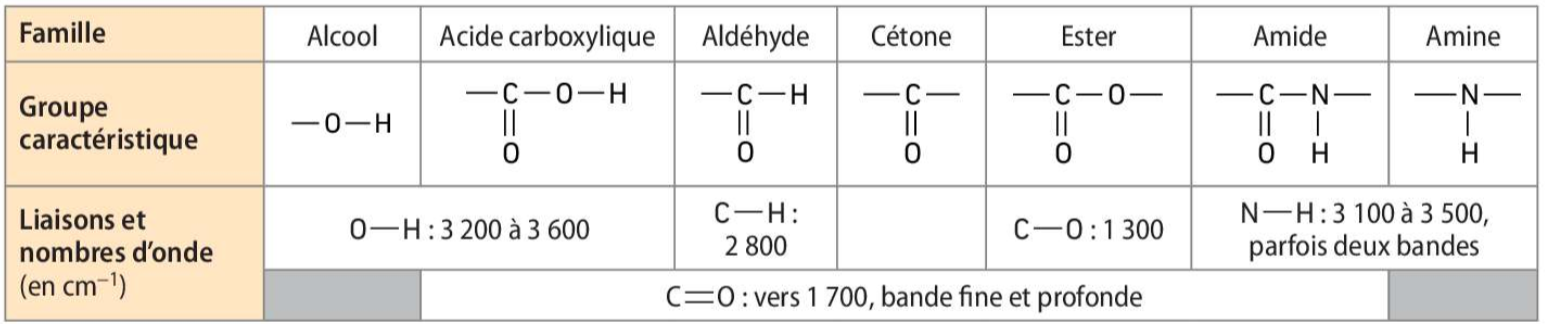
\includegraphics[width=0.9\textwidth]{imgs/c1/IRtable.png}
    \caption{Les bandes d'absorption IR les plus importantes.}
    \label{fig:bandesIR}
\end{figure}

(c.f. Mon cours sur IR de l'ancien programme, si vous voulez voir en plus grande détails les principes et les bandes d'absorption IR)

\section{Conductimétrie}

La conductimétrie est une autre méthode de détermination de la concentration d'une solution, en exploitant ses propriétés physico-chimiques; ici les propriétés électriques de la solution. Nous allons donc trouver une relation (la loi de Kohlrauch) analogue à la relation de Beer-Lambert, nous donnant une relation linéaire entre la concentration de la solution en ions, et la propriété que l'on verra par la suite, la \textbf{conductance} de la solution.

\subsection{Conductance, conductivité \& la cellule conductimétrique}

\begin{defn}{Conductance}

La conductance $G$ d’une portion de la solution électrolytique est, par définition, égale à l’inverse de la résistance $R$ de la même portion.  
\[  G=\dfrac{1}{R}    \text{\quad où \quad} \begin{cases}
     G \rightarrow \text{Conductance en siemens }(S) \\
     R \rightarrow \text{Résistance en ohms }(\Omega) \\ 
     \end{cases}
  \]
\end{defn}
\begin{exo}
Donner la loi d’Ohm avec la conductance au lieu de la résistance. 
\vspace{1cm}
Déterminer la conductance entre deux armatures ayant une tension de $2\; V$, traversées par un courant d'intensité $I=0,35\; A$. 
\vspace{1.3cm}
\end{exo}

\begingroup
\setlength{\intextsep}{0pt}%
\setlength{\columnsep}{5pt}%

\begin{wrapfigure}{r}{0.25\textwidth}
  \centering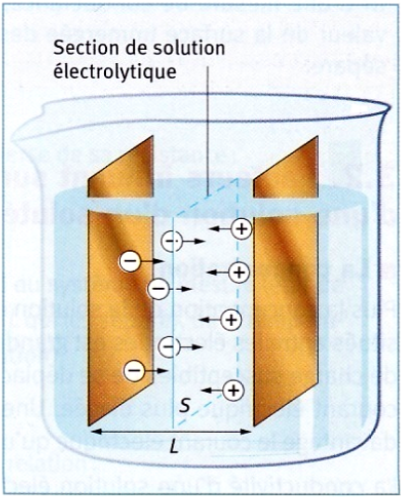
\includegraphics[width=\linewidth]{imgs/c1/celluleconducti.png}
  \caption{Cellule conductimétrique.}
\end{wrapfigure}

Comment peut-on alors mesurer cette conductance de la solution ?

Cela se fait grâce à une « cellule conductimétrique ».  Cette cellule est constituée de deux plaques métalliques (i.e. deux électrodes), cuivre ou platine, planes et parallèles, d’une surface $S$, séparées d’une distance $\ell$. 

Le conductimètre impose une tension électrique $U$ entre ces deux plaques, puis mesure l'intensité du courant $I$ qui s'établit; ce qui permet la détermination de la conductance $G$ grâce à la loi d'Ohm 
$$I= G\cdot U \quad \Leftrightarrow \quad G=\frac{I}{U}$$  

Quels sont les facteurs qui influencent une cellule conductimétrique ?

\endgroup

Les paramètres influençant la cellule sont tous géométriques.
\begin{itemize}
    \item Plus la surface immergée $S$ des électrodes est grande, plus y a d’ions susceptibles de passer d’une électrode à l’autre. c'est-à-dire $G \propto S $.
    \item Plus la distance $\ell$ séparant les électrodes est grande, moins il y a d’ions capables de parcourir cette distance. c'est-à-dire $G \propto \frac{1}{\ell} $.
\end{itemize}
	 
En conclusion on peut donc dire : $G \propto \frac{S}{\ell}$. Afin de passer d'une proportionnalité à une égalité, il faut introduire une constante de proportionnalité, ici nommé $\sigma$, et donc 
\[ G = \dfrac{S}{\ell}\cdot \sigma = k\cdot \sigma      \]

\begin{defn}{Conductivité}
\begin{itemize}
    \item La constante $\sigma$ représente la \textbf{conductivité} \eng{conductivity} de la solution.   
    \item La conductivité d’une solution est une mesure de son aptitude à conduire le courant électrique.  Elle est \textbf{caractéristique de la solution}, et donc ne dépend que des facteurs physico-chimiques relatifs à la solution. 
    \item Elle s’exprime en $S\cdot m^{-1}$ avec la surface $S$ en $m^2$ , et la distance $\ell$ en $m$.  Souvent les unités sont exprimées en $cm$ au lieu de $m$.
    \item La constante $k=\frac{S}{\ell}$ s’appelle la \textbf{constante de la cellule}, et caractérise la cellule conductimétrique. 
\end{itemize}
\end{defn}
\vspace{1cm}
Voici les facteurs principaux qui influencent la conductivité d'une solution : 

\begin{itemize}
    \item \textbf{Concentration}
    
    C’est la présence de l’électrolyte qui rend la solution conductrice.  N’oublions pas que le courant électrique dans une solution est dû à un double courant d’ions.  Plus la concentration est élevée, plus il y a d’ions entre les électrodes. La conductivité est d’autant plus grande donc que la solution est concentrée.  
    \item \textbf{Température}
    
    La température – comme d’habitude – entre aussi en jeu.  Plus la température est  élevée plus la conductivité est grande. Ceci est - comme vous l'avez \textit{sans doute} deviné - lié à l'agitation thermique du milieu (c.f. remarque ci-après). 
    
    \item \textbf{Nature des ions}
    
    Les ions peuvent se distinguer par leur charge, par leur taille, par le nombre de molécules de solvant qui les solvatent, etc.  Lors de leurs déplacements, ils ne sont pas freinés de la même façon, d’où leurs différentes aptitudes à conduire le courant électrique. 
\end{itemize}
\begin{rmrq}
La température est une mesure d’agitation thermique, c'est-à-dire, le mouvement des ions/molécules dans la solution.  Plus la température est élevée, plus les ions se déplacent facilement, et donc la conductivité augmente.  Par conséquent, il est impératif de maintenir une température constante lors des mesures de conductance. 
\end{rmrq}

\subsection{Loi de Kohlrauch}
On se rappelle que le passage du courant électrique dans une solution électrolytique est dû a un \textit{double courant d’ions}, les anions dans un sens et les cations, dans le sens inverse.  

On représente ce fait, mathématiquement, avec une relation simple : $\sigma= \sigma_+ + \sigma_-$  où $\sigma_+$  représente la conductivité des cations et $\sigma_-$ celle des anions. 

De plus, on sait que la conductivité d’un ion à une température donnée dépend de sa concentration en solution ainsi que de sa nature.  Donc, pour un cation quelconque $\ce{M_{(aq)}^+}$, on peut dire que :

$\sigma_{\ce{M_{(aq)}^+}}= \lambda_{\ce{M_{(aq)}^+}}\cdot[\ce{M_{(aq)}^+}]$
où $[\ce{M_{(aq)}^+}]$ donne la concentration en solution de l’ion, et le symbole $\lambda_{\ce{M_{(aq)}^+}}$ est une nouvelle grandeur qui s’appelle la conductivité molaire ionique de $[\ce{M_{(aq)}^+}]$.

\begin{defn}{Conductivité molaire ionique}
\begin{itemize}
    \item À chaque ion $ \ce{X} $ d’une solution ionique on a affecté une \textbf{conductivité molaire ionique} $ \lambda_X $ qui le caractérise.  
    \item Elle s’exprime en $S\cdot m^2\cdot mol^{-1}$.  
    \item Elle dépend de la température de la solution, et de la nature du solvant.  
\end{itemize}
\end{defn}

Chaque ion contribue à la conductivité de la solution en fonction de sa concentration et de sa conductivité molaire ionique. 

La conductivité totale de la solution (dans la limite des concentrations faible) est donnée par la somme des chacune de ses contributions : c'est\textbf{ la loi de Kohlrausch}. 
\newpage
Pour une solution contenant $p$ ions différents, la conductivité de la solution est donnée par :

\begin{shaded}
\[ 
\sigma = \sum^p_i \lambda_i\cdot[\ce{X_i}] \quad où \quad
     \begin{cases}
     \sigma \rightarrow \text{conductivité de la solution }(S\cdot m^{-1}) \\
     \lambda_i \rightarrow \text{conductivité molaire ionique de l'espèce $\ce{X_i}$ }(S\cdot m^2\cdot mol^{-1}) \\
     [\ce{X_i}] \rightarrow \text{concentration molaire de l'espère $\ce{X_i}$ }(mol\cdot m^{-3})
     \end{cases} 
\]     
\end{shaded}

\begin{rmrq}
La loi de Kohlrausch n'est valable que pour des concentrations $\leq 10^{-2}\mpl$.
\end{rmrq}

\begin{figure}[h]
    \centering
    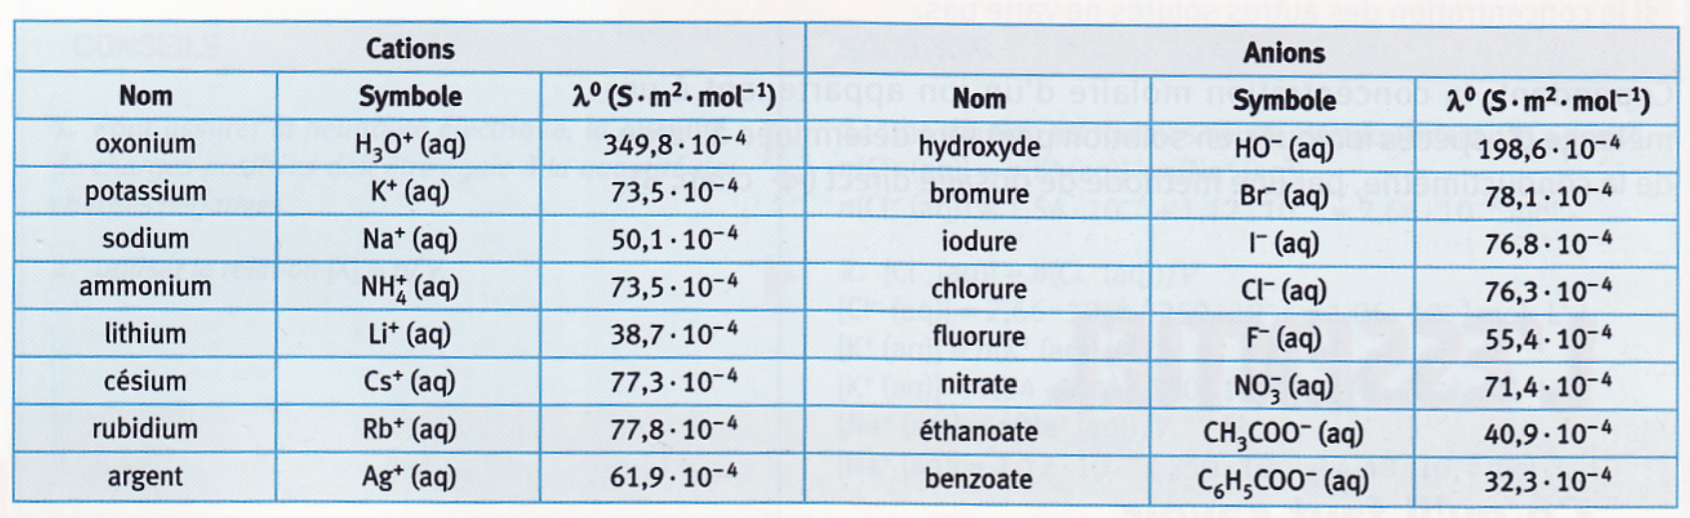
\includegraphics[width=\textwidth]{imgs/c1/lambdaTable.png}
    \caption{Conductivité molaire ionique de quelques ions, en solution diluée, à $25\degree$}
\end{figure}

\section{Dosages}

Allons droit au but : 
\begin{itemize}
    \item \textbf{Le but d’un dosage est de déterminer la concentration molaire d’une solution inconnue, en la faisant réagir avec une autre solution dont la concentration est connue.}
    \item La solution dont la concentration est inconnue et qui est dosée s’appelle la \textbf{solution titrée}. Le réactif titré est l’espèce dosée dans la solution titrée. 
    \item La solution versée et qui réagit avec la solution titrée, dont la concentration est connue a priori, s’appelle la \textbf{solution titrante}. Elle contient le réactif titrant.
\end{itemize}

\subsection{Dosage par titrages}

Caractérisons donc d’abord les types de réactions nécessaires pour un titrage \eng{titration} . La transformation qui résulte de l’addition d’une solution titrante est modélisée par une réaction chimique, la réaction du dosage.  Cette réaction doit être :

\begin{itemize}
    \item \textbf{Rapide} : c'est-à-dire qu’elle parvient à son terme soit de manière instantanée, soit dans un temps bref.
    \item \textbf{Totale} : le réactif limitant est toujours totalement consommé.
    \item \textbf{Spécifique (univoque)} : c'est-à-dire non perturbée par une autre réaction ayant les mêmes réactifs mais des produits différents. 
    \item \textbf{Observable} : c'est-à-dire la transformation doit présenter une caractéristique physique, observable, variant au cours du temps du titrage et facilement mesurable.
\end{itemize}

\subsubsection{Exemple d'un titrage}

\begingroup
\setlength{\intextsep}{10pt}%
\begin{wrapfigure}{r}{0.5\textwidth}
  \centering
  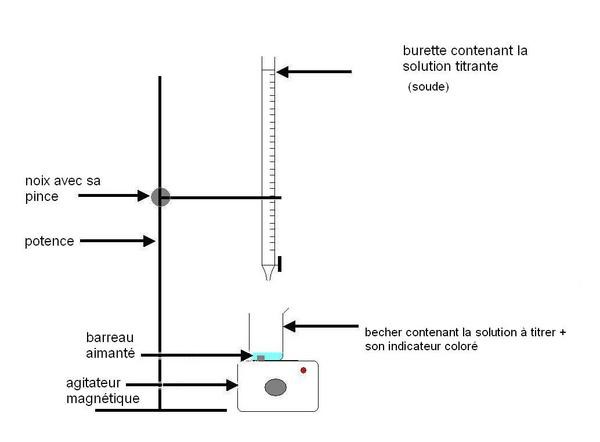
\includegraphics[width=.95\linewidth]{imgs/c1/montage.jpg}
  \caption{Montage typique d'un dosage}
\end{wrapfigure}

Expérimentalement
\begin{itemize}
    \item afin de pouvoir mesurer précisément le volume versé de la solution titrante, on utilise une \textbf{burette}.  
    \item Il est très important d’\textbf{agiter la solution} lors du dosage, afin de l'homogénéiser.
\end{itemize}

Considérons l’expérience suivante :

Un récipient contient un volume $V$ d’une solution de sulfate de fer $\left(\ce{Fe^{2+}_{(aq)} + SO^{2-}_{4 (aq)}}\right)$ et donc des ions de fer (II) $\ce{Fe^{2+}_{(aq)}}$, une solution incolore. 

On introduit continuellement une solution de permanganate de potassium $\left(\ce{K^{+}_{(aq)} + MnO4^{-}_{(aq)}}\right)$, qui contient des ions de permanganate $\ce{MnO4^{-}_{(aq)}}$, formant une solution violette. 

\endgroup

\textbf{Qu'observe-t-on lors de l'expérience, au niveau de l'aspect de la solution du mélange?}  

Comme dans la figure ci-après, au début, le mélange reste incolore, même si le permanganate a une couleur violette très distincte (images I et II). À partir d'un instant, les gouttes violettes maintiennent leurs couleurs et la solution devient colorée, et de manière permanente (image III). 

\begin{figure}[h]
    \centering
    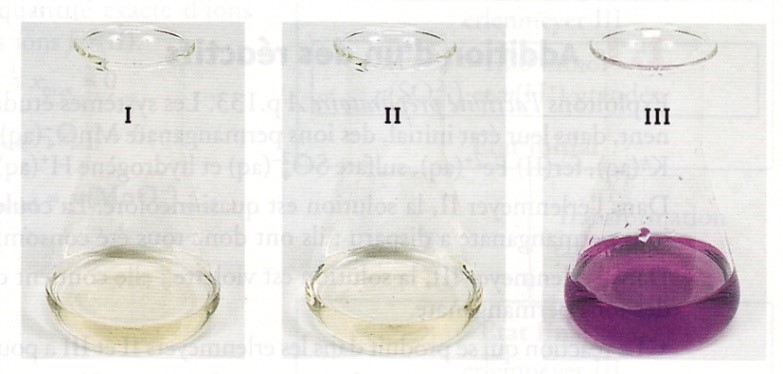
\includegraphics[width=0.8\linewidth]{imgs/c1/fer.jpg}
    \caption{Le dosage des ions fer (II) par des ions permanganate.}
    \label{fig:dosagefer}
\end{figure}


\textbf{Comment expliquer et interpréter ces observations alors?}  

Revenons à nos réactions classiques et statiques.  En considérant notre mélange réactionnel nous pouvons avoir une de ces trois conditions :

\begin{enumerate}
	\item L’ion de permanganate est le réactif limitant : $\ce{MnO4^{-}_{(aq)}}$ s’épuise d’abord, et donc la solution à la fin contient toujours un peu du réactif en excès, ici l’ion de fer (II). \textbf{Observation : } La solution reste incolore, caractéristique des ions Fer (II) présents en solution. 
    \item 	L’ion de fer (II) est le réactif limitant : $\ce{Fe^{2+}_{(aq)}}$ s’épuise d’abord et donc la solution à la fin contient toujours un peu du réactif en excès, ici l’ion permanganate. \textbf{Observation : } La solution a une couleur violette, caractéristique des ions permanganate. 
    \item Les réactifs sont en \textbf{proportions stœchiométriques}, c'est-à-dire, les deux réactifs s’épuiseront au même moment, et donc à la fin de la réaction il ne restera que du produit. \textbf{Observation : } La solution reste incolore, car seul les ions permangante ont une couleur (à vous de vérifier en déterminant la réaction rédox entre les ions permanganate et fer (II) ) . 
\end{enumerate}

Si l'on fait la correspondance entre les trois états énumérés précédemment et la Figure \ref{fig:dosagefer}, l'image I correspond à l'état 1 (les ions fer en excès), l'image II correspond à l'état 2(réactifs on proportions st\oe chiométriques), et l'image III correspond à l'état 3 (permanganate en excès). 

On en fait donc les conclusions suivantes :

\begin{itemize}
    \item \textbf{Le réactif limitant change} selon la valeur du volume de la solution titrante ajoutée. 
    \item En versant la solution de $\ce{MnO4^{-}_{(aq)}}$ continuellement, on passe par trois régimes.  
    \begin{itemize}
        \item Dans un premier temps, le réactif limitant est le permanganate qui est consommé instantanément au contact avec le réactif en excès, qui est le fer (II), d’où la couleur transparente de la solution;
        \item En continuant de verser du permanganate on consomme aussi les ions de Fer (II), et donc la teneur de solution titrée en $\ce{Fe^{2+}_{(aq)}}$ diminue aussi.  À un moment, le $\ce{Fe^{2+}_{(aq)}}$  sera totalement consommé.  Désormais c’est le permanganate le réactif en excès, et donc si l’on continue d’en verser, au lieu d’être consommé, il restera dans la solution, d’où la couleur violette de la solution (due aux ions permanganates qui n’ont pas réagis).  
        \item Il y a un moment unique où le mélange réactionnel sera en proportion stœchiométrique. \textbf{Ce point très important est l’équivalence}. 
    \end{itemize}
\end{itemize}

\begin{defn}{Equivalence}
\begin{itemize}
    \item L’équivalence est définie et caractérisée par le changement de réactif limitant.
    \item Le volume $V_{eq}$  de solution titrante versé à l’équivalence s’appelle le volume à l’équivalence, ou le volume équivalent.
    \item À l’équivalence, les réactifs sont en proportions stœchiométriques.
    \item À l’équivalence, le réactif titré et le réactif titrant ont été totalement consommés.  La solution ne contient que des produits. 
\end{itemize}
\end{defn}

L’équivalence est le seul moment où on peut utiliser les coefficients stœchiométriques afin de déterminer la concentration inconnue de la solution titrée.  

Dans la réaction entre les ions de fer (II) et les ions permanganate, les couples rédox mis en jeu sont :

\[ \ce{MnO4^{-}_{(aq)} / Mn^{2+}_{(aq)} } \quad et \quad   \ce{Fe^{3+}_{(aq)} / Fe^{2+}_{(aq)}}    \]

La réaction d'oxydoréduction entre les deux est donc : 
\begin{shaded}
\vspace{1cm}
\end{shaded}

On se rappelle que $[\MnO]=C_2$ est connue, alors que $[\ce{Fe^{2+}_{(aq)}}]$ est inconnue, et à déterminer grâce au dosage.  

Dressons alors le tableau d’avancement.  Notons que le tableau d’avancement contient des quantités initiales fixes. Pour nous, ces valeurs correspondent aux valeurs à l’équivalence :
\begin{itemize}
    \item La quantité initiale d’ion fer (II) $n_i\left(\ce{Fe^{2+}_{(aq)}}\right) $ est inconnue, et 
    \item La quantité initiale d’ion permanganate $n_i\left(\MnO_{(aq)}\right) $ dépend de la quantité totale versée jusqu’à l’équivalence, donc $n_i\left(\MnO_{(aq)}\right) = n_{versé}\left(\MnO_{(aq)}\right)$.
\end{itemize}

De plus, on ne remplit pas les cases correspondant aux ions $\ce{H+}$  et $\ce{H2O}$ car les quantités de matière de ces deux espèces n’ont pas d’intérêt pour déterminer la concentration recherchée.  Les deux ne seront jamais des réactifs limitants. 

Alors on verse du réactif titrant, jusqu’à ce qu’on arrive à l’équivalence.  À l’équivalence, à l’état final, l’avancement maximal $x_{max}$, peut s’écrire  $x_{éq}$.  De plus on sait que les quantités de matière sont maintenant nulles pour les réactifs, c'est-à-dire (définition de l’équivalence) :

\[ n_{versé}\left(\MnO_{(aq)}\right) - x_{éq} = 0 \quad \text{et} \quad n_i\left(\ce{Fe^{2+}_{(aq)}}\right) - 5 x_{éq} = 0      \]

Or

\[  n_{versé}\left(\MnO_{(aq)}\right) = V_{éq}\cdot C_2  \quad \text{d'où} \quad x_{éq} = V_{éq}\cdot C_2    \]

et on en déduit, 

\[ n_i\left(\ce{Fe^{2+}_{(aq)}}\right) = 5 x_{éq} = 5V_{éq}\cdot C_2       \]

Si on dit que $V_1$ est le volume initial et $C_1$ la concentration initiale de la solution de fer (II) (la concentration inconnue que l'on cherche), on peut maintenant écrire :

\begin{align*}
  n_i\left((\ce{Fe^{2+}_{(aq)}}\right) = V_1\cdot C_1 &= 5V_{éq}\cdot C_2      \\
  C_1 &= \dfrac{5V_{éq}\cdot C_2}{V_1}
\end{align*}

Cet exemple nous permet donc d'établir une règle générale. Pour un dosage par titrage, avec une réaction de support:
\[ \textcolor{blue}{a}\ce{A} + \textcolor{red}{b}\ce{B} \rightarrow c\ce{C} + d\ce{D} \]

À l’équivalence E, les réactifs sont totalement consommés.  C'est-à-dire :

\[ n_i\left( \ce{A}\right) - \textcolor{blue}{a}\cdot x_E = 0 \quad \text{et} \quad  n_i\left( \ce{B}\right) - \textcolor{red}{b}\cdot x_E = 0     \]

D'où

\[ \dfrac{n_i\left( \ce{A}\right)}{\textcolor{blue}{a}} =  \dfrac{n_i\left( \ce{B}\right)}{\textcolor{red}{b}}     \]



Nous voyons clairement que le cas précédent (permanganate et fer (II) ) est bien un cas particulier de cette règle générale. 

\subsection{Détermination de l'équivalence}

D’accord, dites-vous, tout cela est bien beau, mais \textbf{comment peut-on savoir quand on arrive à l’équivalence ? }

Bonne question !  Passons donc à la partie expérimentale, car ce que nous avons vu dans la partie précédente nous montre comment calculer une concentration à partir de la valeur du volume versé pour arriver à l'équivalence, mais la détermination de ce volume est une question plutôt expérimentale. 

D’abord, quand il est possible, on préfère de ne pas \textit{détruire} la solution originale. Nous commençons donc par prélever un volume connu de la solution, dans un bécher par exemple : c’est la \textbf{prise d’essai}. Cette prise d’essai est parfois diluée avant le dosage (en fonction de la méthode expérimentale choisie).  

Dans la partie suivante, nous allons détailler donc les différentes méthodes expérimentales que l'on voit souvent, permettant de repérer le point d'équivalence. Chaque méthode va dépendre du \textbf{choix de l'observable}, c'est-à-dire la caractéristique que l'on peut observer ou mesurer.

\subsubsection{Titrage colorimétrique}

\begin{wrapfigure}{r}{0.45\textwidth}
  \centering
  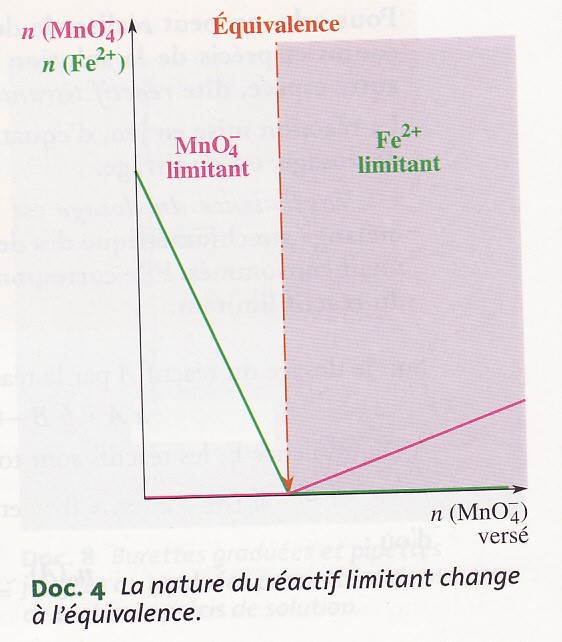
\includegraphics[width=.95\linewidth]{imgs/c1/graphequiv.jpg}
\end{wrapfigure} 

\textbf{L’observable ici est la couleur de la solution} dans le bécher, c'est-à-dire le milieu réactionnel subit un changement de couleur, bien visible. C’est très souvent le cas dans les dosages d’oxydoréduction.  Dans ce cas-là il y a une différence de couleur entre l’oxydant et le réducteur d’un des deux couples.

Par exemple, dans l’expérience où l’on dose une solution de fer (II) par une solution de permanganate, au début la solution est quasi-incolore en raison de la présence d’ions de fer (II) qui sont en excès, donc le permanganate se transforme immédiatement en espèce réductrice (i.e. ion manganèse).  En revanche, dès que l’on dépasse l’équivalence, il n’y a plus d’ions fer (II), les ions permanganate ajoutés à la solution ne réagissent plus. Par conséquent la franchise de l’équivalence se manifeste par un changement de couleur important (les ions permanganate donnent une couleur violette à la solution) (c.f. figure ci-contre). 

Ceci n'est pas le cas de toute solution, et c'est même rarement le cas. Nous pouvons, néanmoins, en \textbf{introduisant un indicateur coloré}, forcer un changement de couleur à l'équivalence. 

Un \textbf{indicateur coloré} est une espèce chimique qui sera choisie de telle façon qu’elle ne prend pas part à la réaction de dosage et qu’elle a la propriété de changer de couleur en même temps que le réactif limitant change.  
Par exemple, le BBT est un indicateur coloré acido-basique.  Le BBT est jaune en présence d’ions oxonium, bleu en présence d’ion hydroxyde.  Donc on peut l’utiliser pour un dosage acido-basique.

\begin{figure}[h]
    \centering
    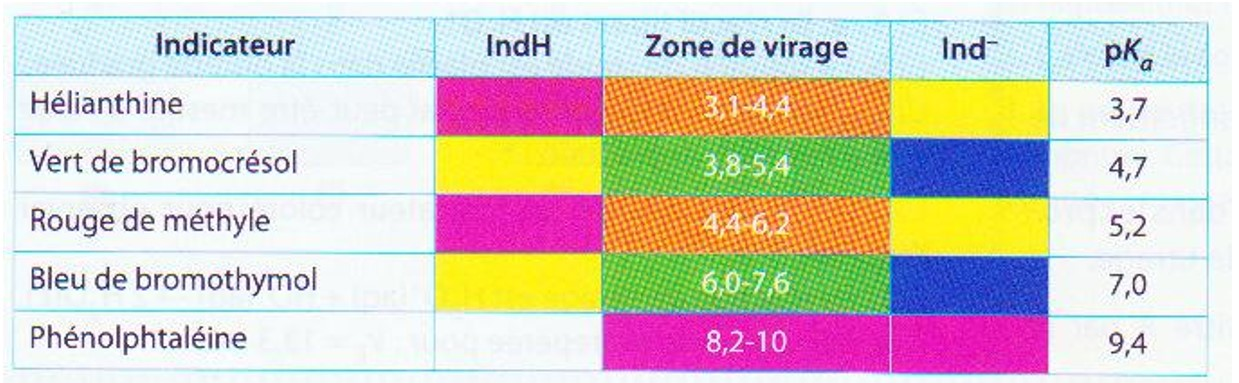
\includegraphics[width=0.8\linewidth]{imgs/c1/indicateurs.jpg}
    \caption{Quelques indicateurs colorés commun (acidobasique).}
\end{figure}
\newpage
\subsubsection{Titrage conductimétrique}
\begingroup
\setlength{\columnsep}{15pt}%
\begin{wrapfigure}{r}{0.4\textwidth}
  \centering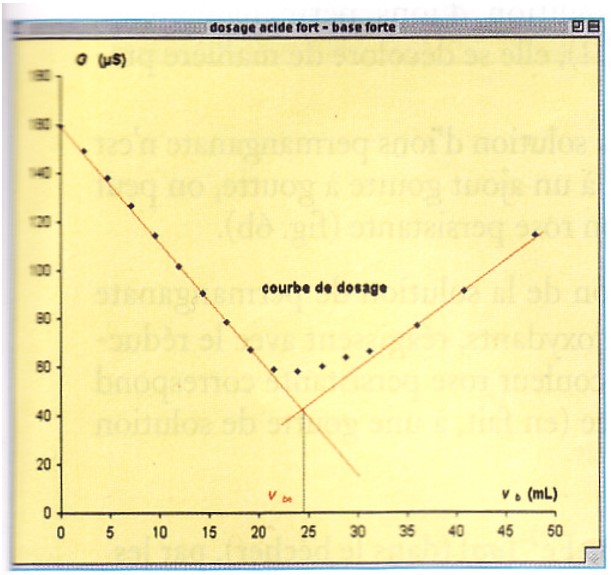
\includegraphics[width=\linewidth]{imgs/c1/courbeV.jpg}
  \caption{Variation de la conductivité d'une solution en fonction du volume de solution titrante versé.}
\end{wrapfigure}
\textbf{L’observable ici est la conductance de la solution}.   Que le dosage soit acido-basique, ou rédox, la solution contiendra des espèces chargées. En suivant l'évolution de la conductance (ou la conductivité de la solution), nous pouvons repérer quand il y a un changement du réactif limitant. 

Par exemple, si la réaction de dosage est une réaction acido-basique entre les ions oxonium et les ions hydroxyde, la réaction entre les deux réduira la teneur de la solution en particules chargées, et donc en approchant l’équivalence, la conductance devrait diminuer (fonction décroissante).  À l’équivalence alors, la conductance atteindra une valeur minimale.  

Après l’équivalence, la conductance est une fonction croissante, car l’absence des ions hydroxyde (totalement consommés) veut dire qu’en continuant le dosage, on y rajoute des ions oxonium et donc la conductance augmente.  
Afin de déterminer le volume à l’équivalence, on détermine graphiquement le volume correspondant à la conductance minimale.  

\endgroup

\subsubsection{Titrage pH-métrique}

Lors d’un titrage pH-métrique, le $pH$ est mesuré après chaque ajout de solution titrante. Contrairement à un titrage avec un indicateur coloré, la solution titrante continue à être versée au-delà de l’équivalence (car l'équivalence ne peut être déterminé qu'après la fin du dosage et grâce à une analyse des résultats). 

Nous obtenons de cette manière des $pH$ en ordonnées et des volumes en abscisses, qui nous donnent après avoir été reportés dans un graphique, la courbe du titrage acido-basique (cf. figure ci-après). 

Une fois la courbe $pH = f\left(V_{versé}\right)$ obtenu, nous pouvons analyser graphiquement la courbe afin de glaner différentes informations: 

\begin{itemize}
    \item La partie AB où les variations des $pH$ sont assez faibles, avant l’équivalence, 
    \item La partie BC, appelée « la \textbf{zone de virage} » ou « le \textbf{saut de $pH$} », où se trouve le point d’équivalence, 
    \item La partie CD où le $pH$ se stabilise, après l’équivalence. 
\end{itemize}

\begin{figure}[h]
    \centering
    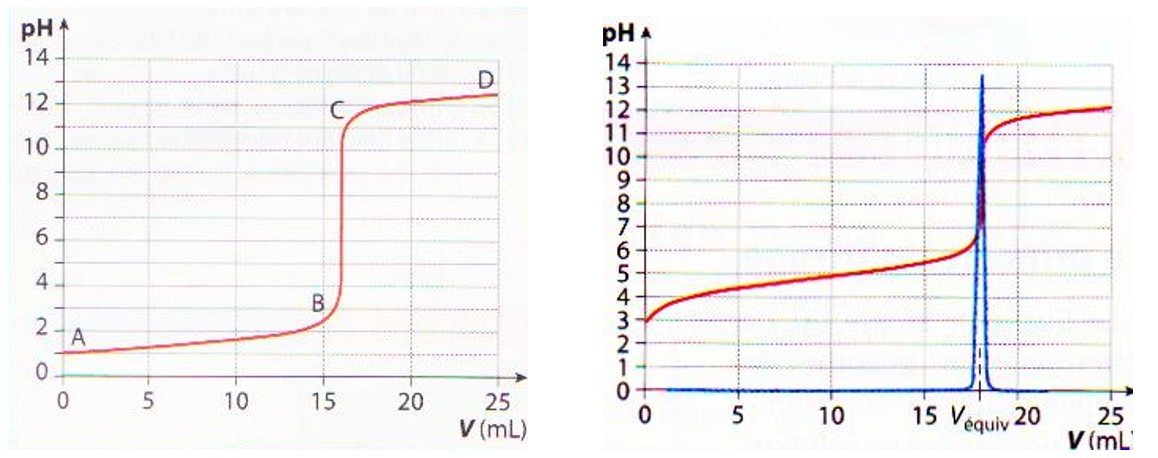
\includegraphics[width = \linewidth]{imgs/c1/methodederive.jpg}
    \caption{Une courbe d'évolution du $pH$ d'une solution acide par une base (gauche); détermination de l'équivalence par la méthode des dérivés (droite).}
    \label{fig:courbespH}
\end{figure}

Le volume versé à l'équivalence, correspond à l'abscisse du \textbf{point d'inflexion} de la courbe $pH=f(V)$.

Pour trouver le point d’équivalence à partir de cette courbe, on se sert de deux méthodes différentes : 
\begin{itemize}
    \item \textbf{Méthode de la courbe dérivée }: la courbe étant le pH en fonction du volume versé, $pH=f(V)$, sa courbe dérivée $g(V)=\od{pH}{V} $ caractérise les \textbf{variations} du $pH$ par rapport au volume versé.  L’équivalence correspond à l’extremum de la courbe dérivée (cf. figure ci-avant à droite). Le volume à l’équivalence correspond donc à l’abscisse de l’extremum. 
    \item \textbf{Méthode des tangentes (c.f. fiche méthode dans le manuel) : }
    \begin{itemize}
        \item Tracer d’abord deux tangentes à la courbe $pH=f(V)$, parallèles entre elles et situées avant et après le saut du $pH$.
        \item Tracer ensuite la parallèle à ces deux tangentes, équidistante de celles-ci.  Son intersection avec la courbe $pH=f(V)$ détermine le point équivalence sur la courbe.
    \end{itemize}
\end{itemize}

\begin{figure}[h]
    \centering
    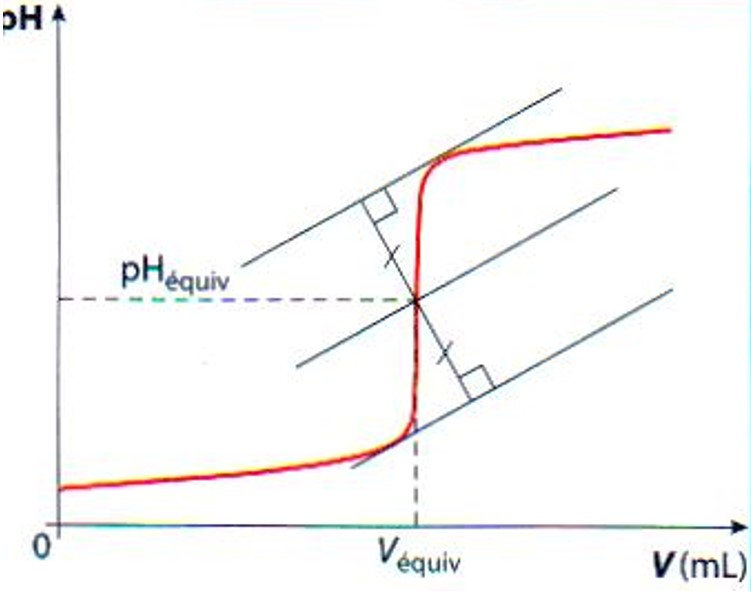
\includegraphics[width=0.55\linewidth]{imgs/c1/methodetangente.jpg}
\end{figure}

\subsection{Dosage par étalonnage}

Nous avons déjà vu comment exploiter une courbe d'étalonnage depuis la classe de seconde. L'idée est très simple : établir une relation entre la concentration et et une grandeur mesureable (absorbance, conductivité, etc), grâce à a des solutions étalons préparées avec des concentrations connues. Etablissons en suite la \textbf{courbe d'étalonnage} (grandeur mesurée en ordonnée, concentration en abscisse). Finalement, on peut exploiter cette courbe pour toute mesure de concentration inconue. Voici un exemple : 

On a déjà établi qu’il existe une relation de proportionnalité entre la conductance et la concentration d’ions.  C’est une relation implorante : elle nous permet de mesurer, indirectement, la concentration d’une solution. 
Pour des concentrations inférieures à $10^{-2}\mpl$ la relation est une droite (i.e. Linéaire).  La courbe $G=f(c)$, est une droite passant quasiment par l’origine, qui s’appelle la courbe d’étalonnage (que l’on construit en mesurant la conductance G pour des variations de la concentration de l’ion).  

On l’utilise alors pour trouver les concentrations inconnues.  On mesure la conductance avec le conductimètre, puis on se rapporte à la courbe d’étalonnage et on lit la concentration correspondant à la conductance mesurée. 

\begin{figure}[h]
    \centering
    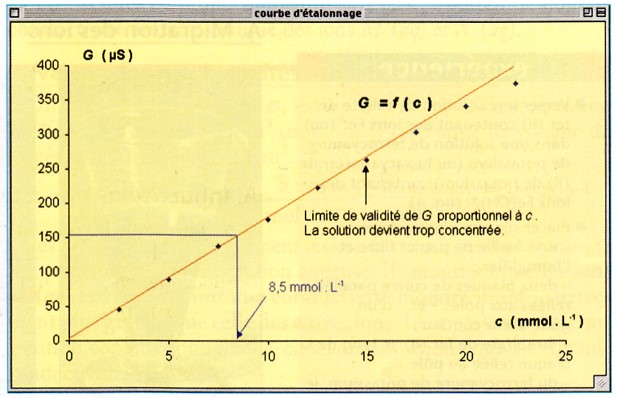
\includegraphics[width=0.8\linewidth]{imgs/c1/etalonnage.jpg}
\end{figure} 

Cependant, cette méthode a des limites :
\begin{itemize}
    \item La relation est linéaire seulement pour des concentrations faibles.  Au-delà la courbe n’est plus droite
    \item Cette méthode marche lorsqu’il n’y a qu’un seul ion dans la solution.  Dans une solution contenant un mélange de plusieurs ions, la conductivité dépend de la concentration de plusieurs ions.
\end{itemize}
\newpage	 
\section{Exercices Résolus}	 

\begin{figure}[h]
    \centering
    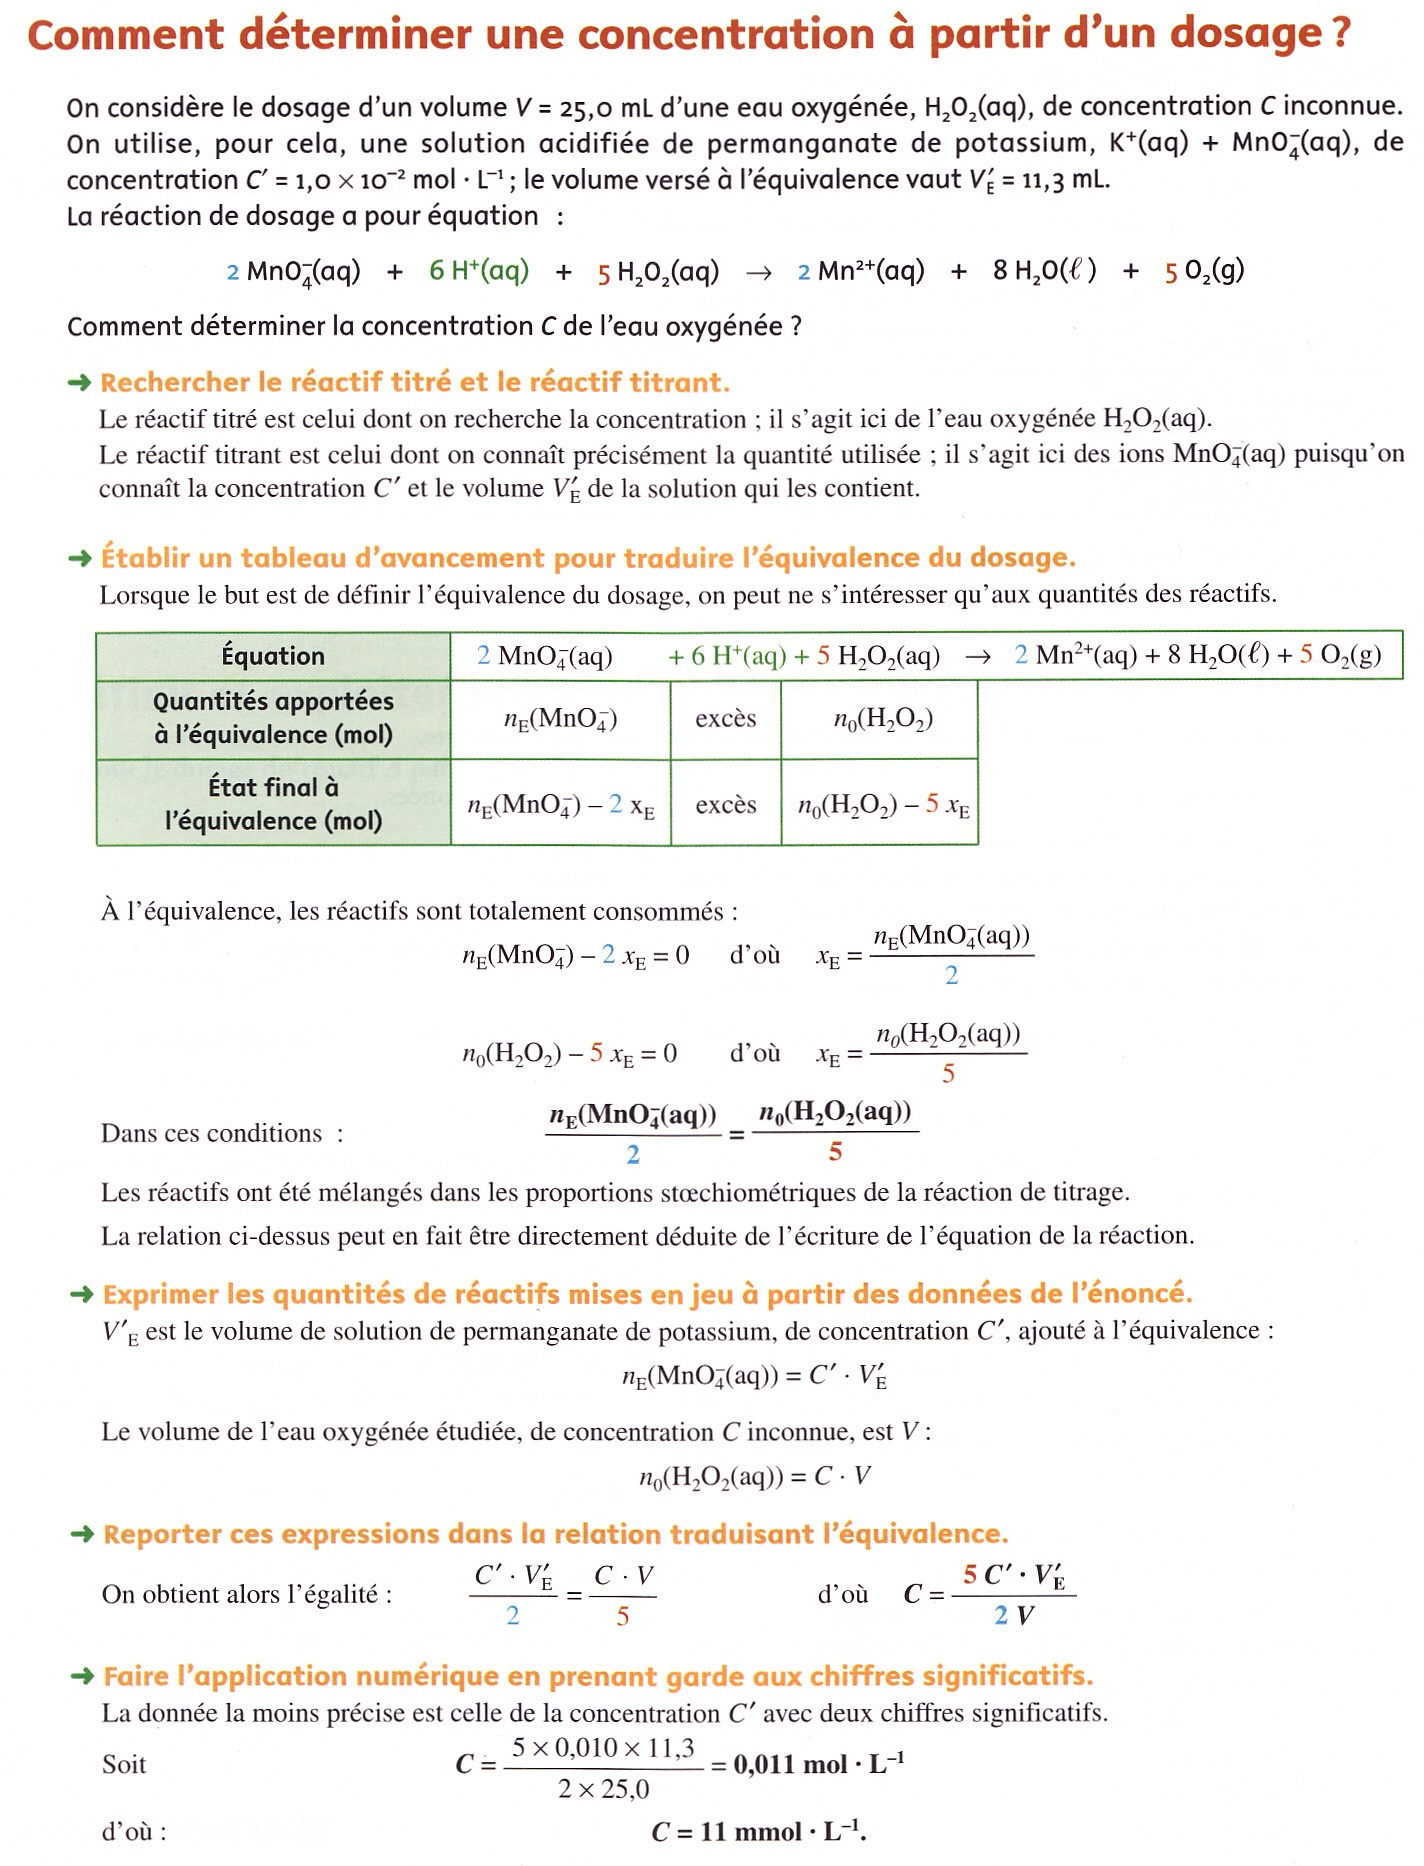
\includegraphics[width=.85\linewidth]{imgs/c1/xo1.jpg}
\end{figure}  

\begin{figure}[h]
    \centering
    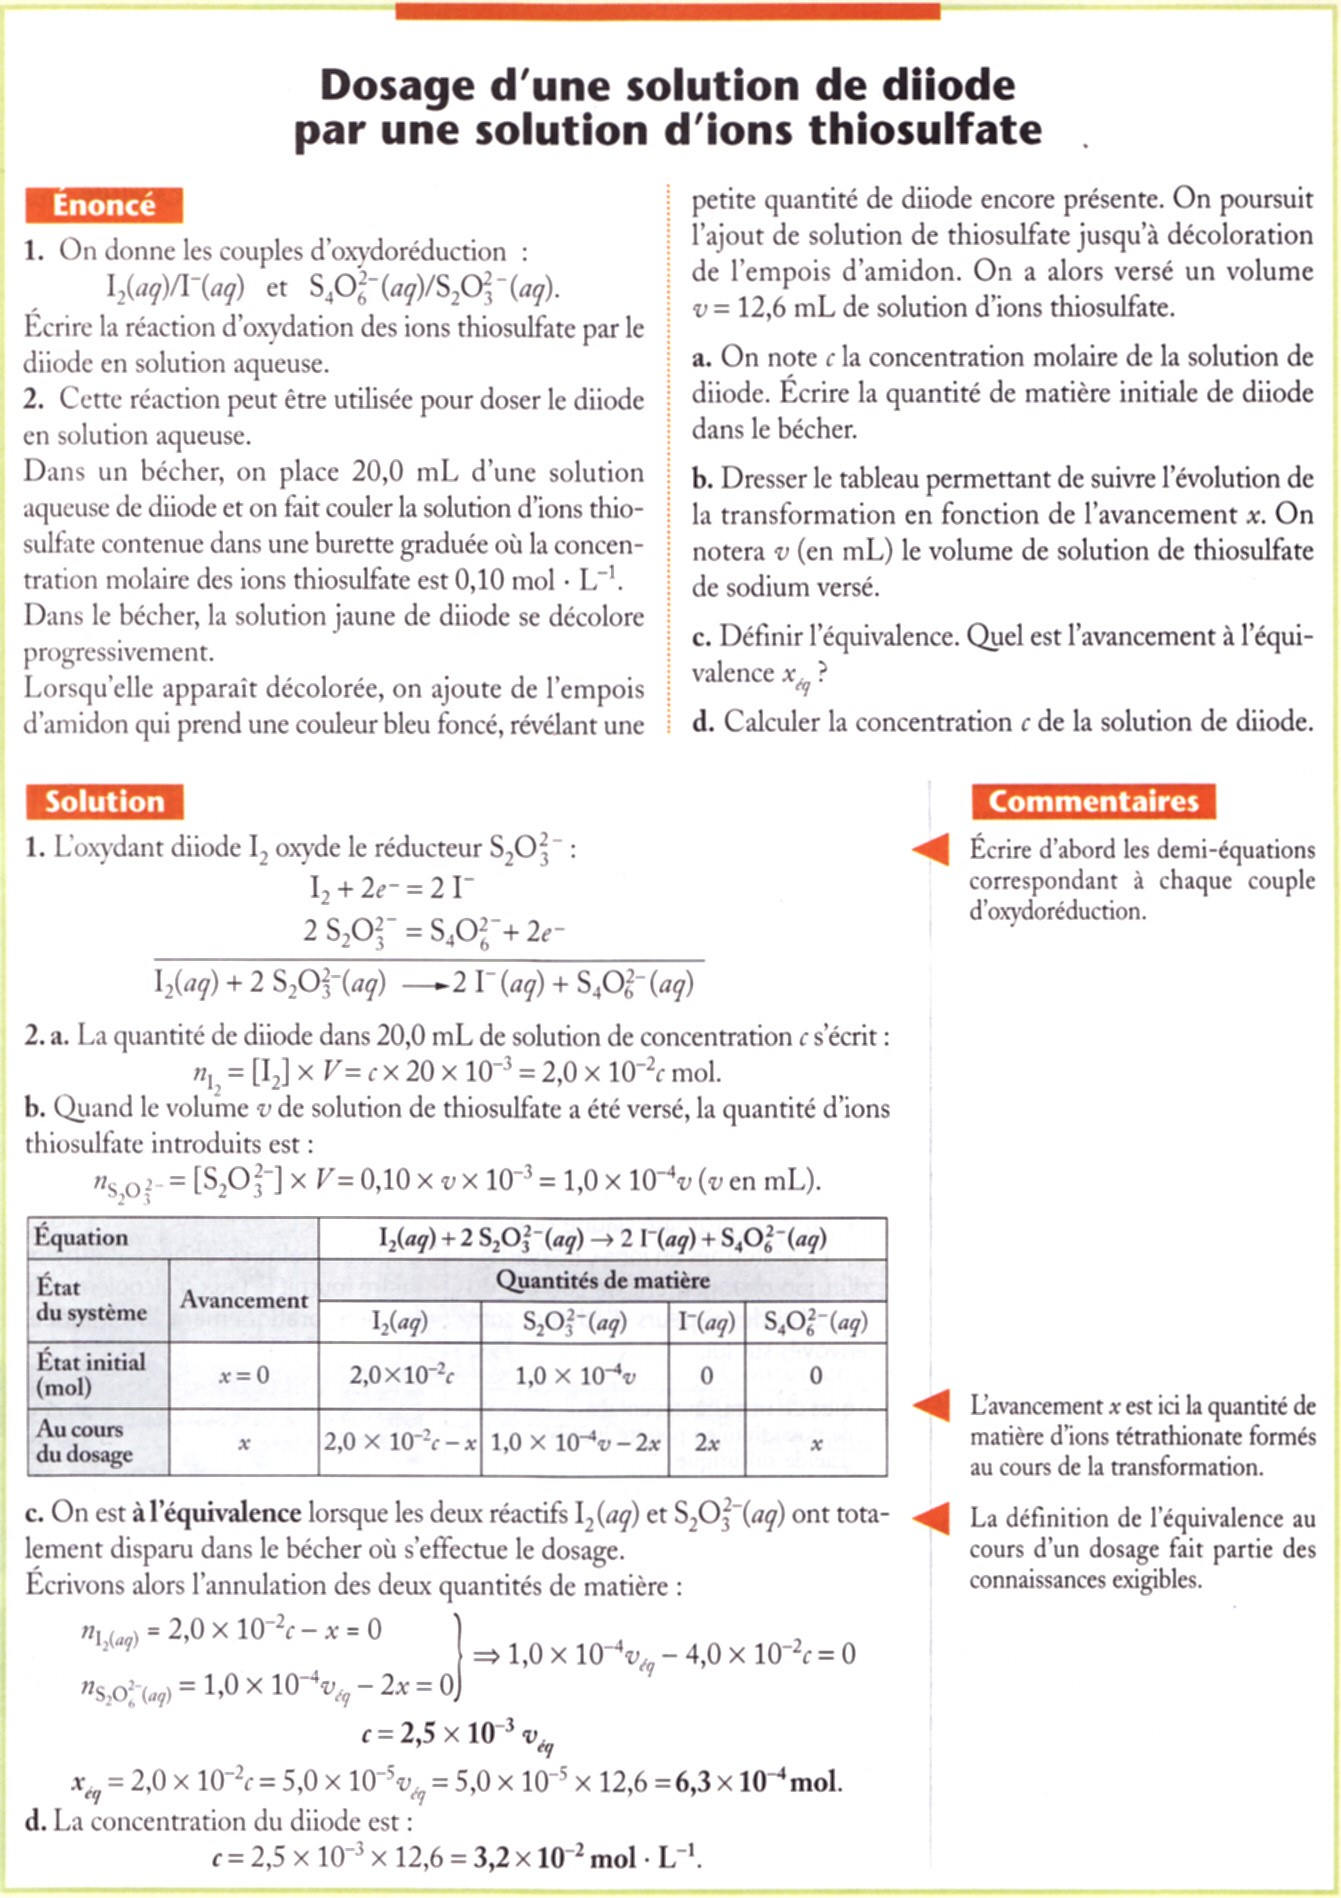
\includegraphics[width=\linewidth]{imgs/c1/xo2.jpg}
\end{figure} 

\begin{figure}[h]
    \centering
    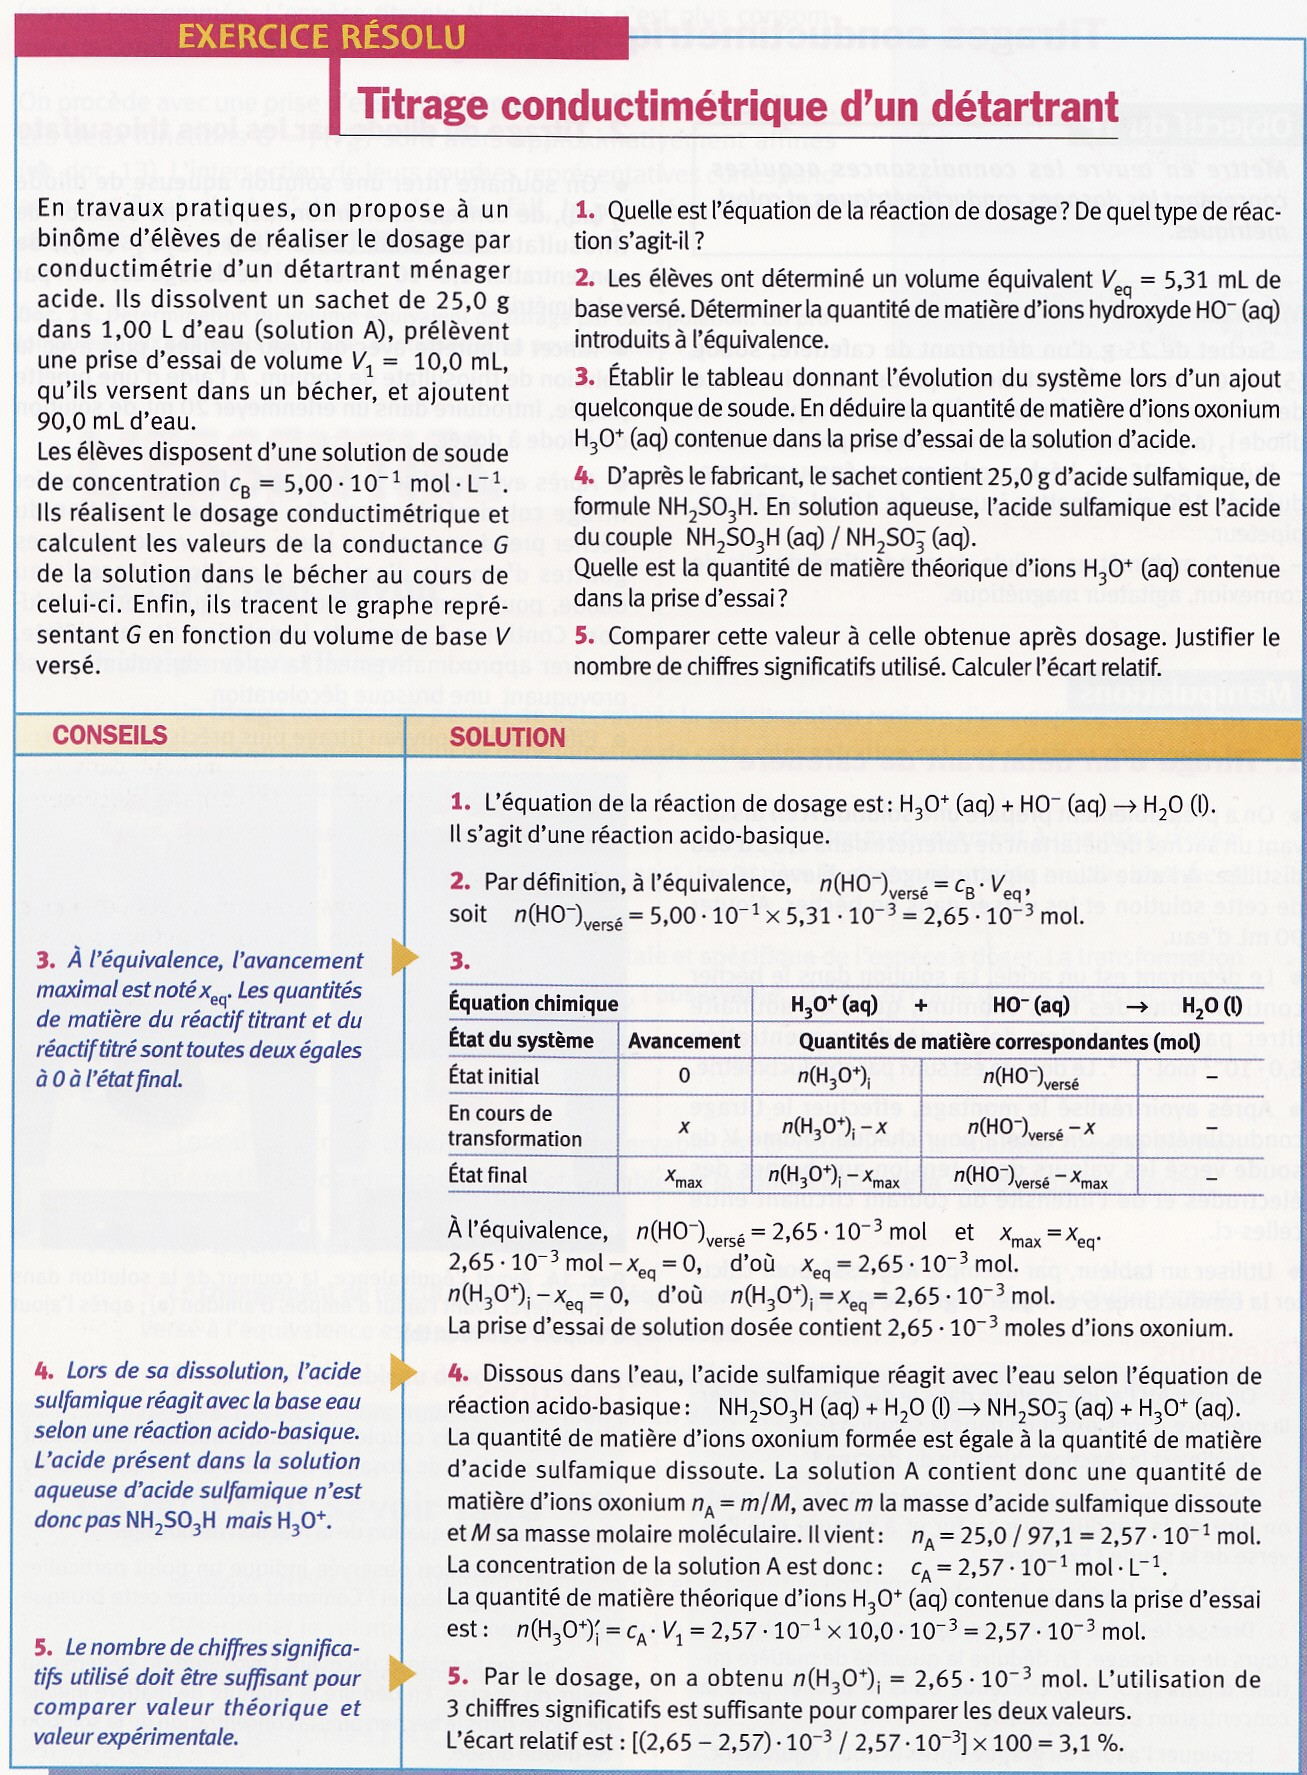
\includegraphics[width=\linewidth]{imgs/c1/xo3.jpg}
\end{figure} 

\begin{figure}[h]
    \centering
    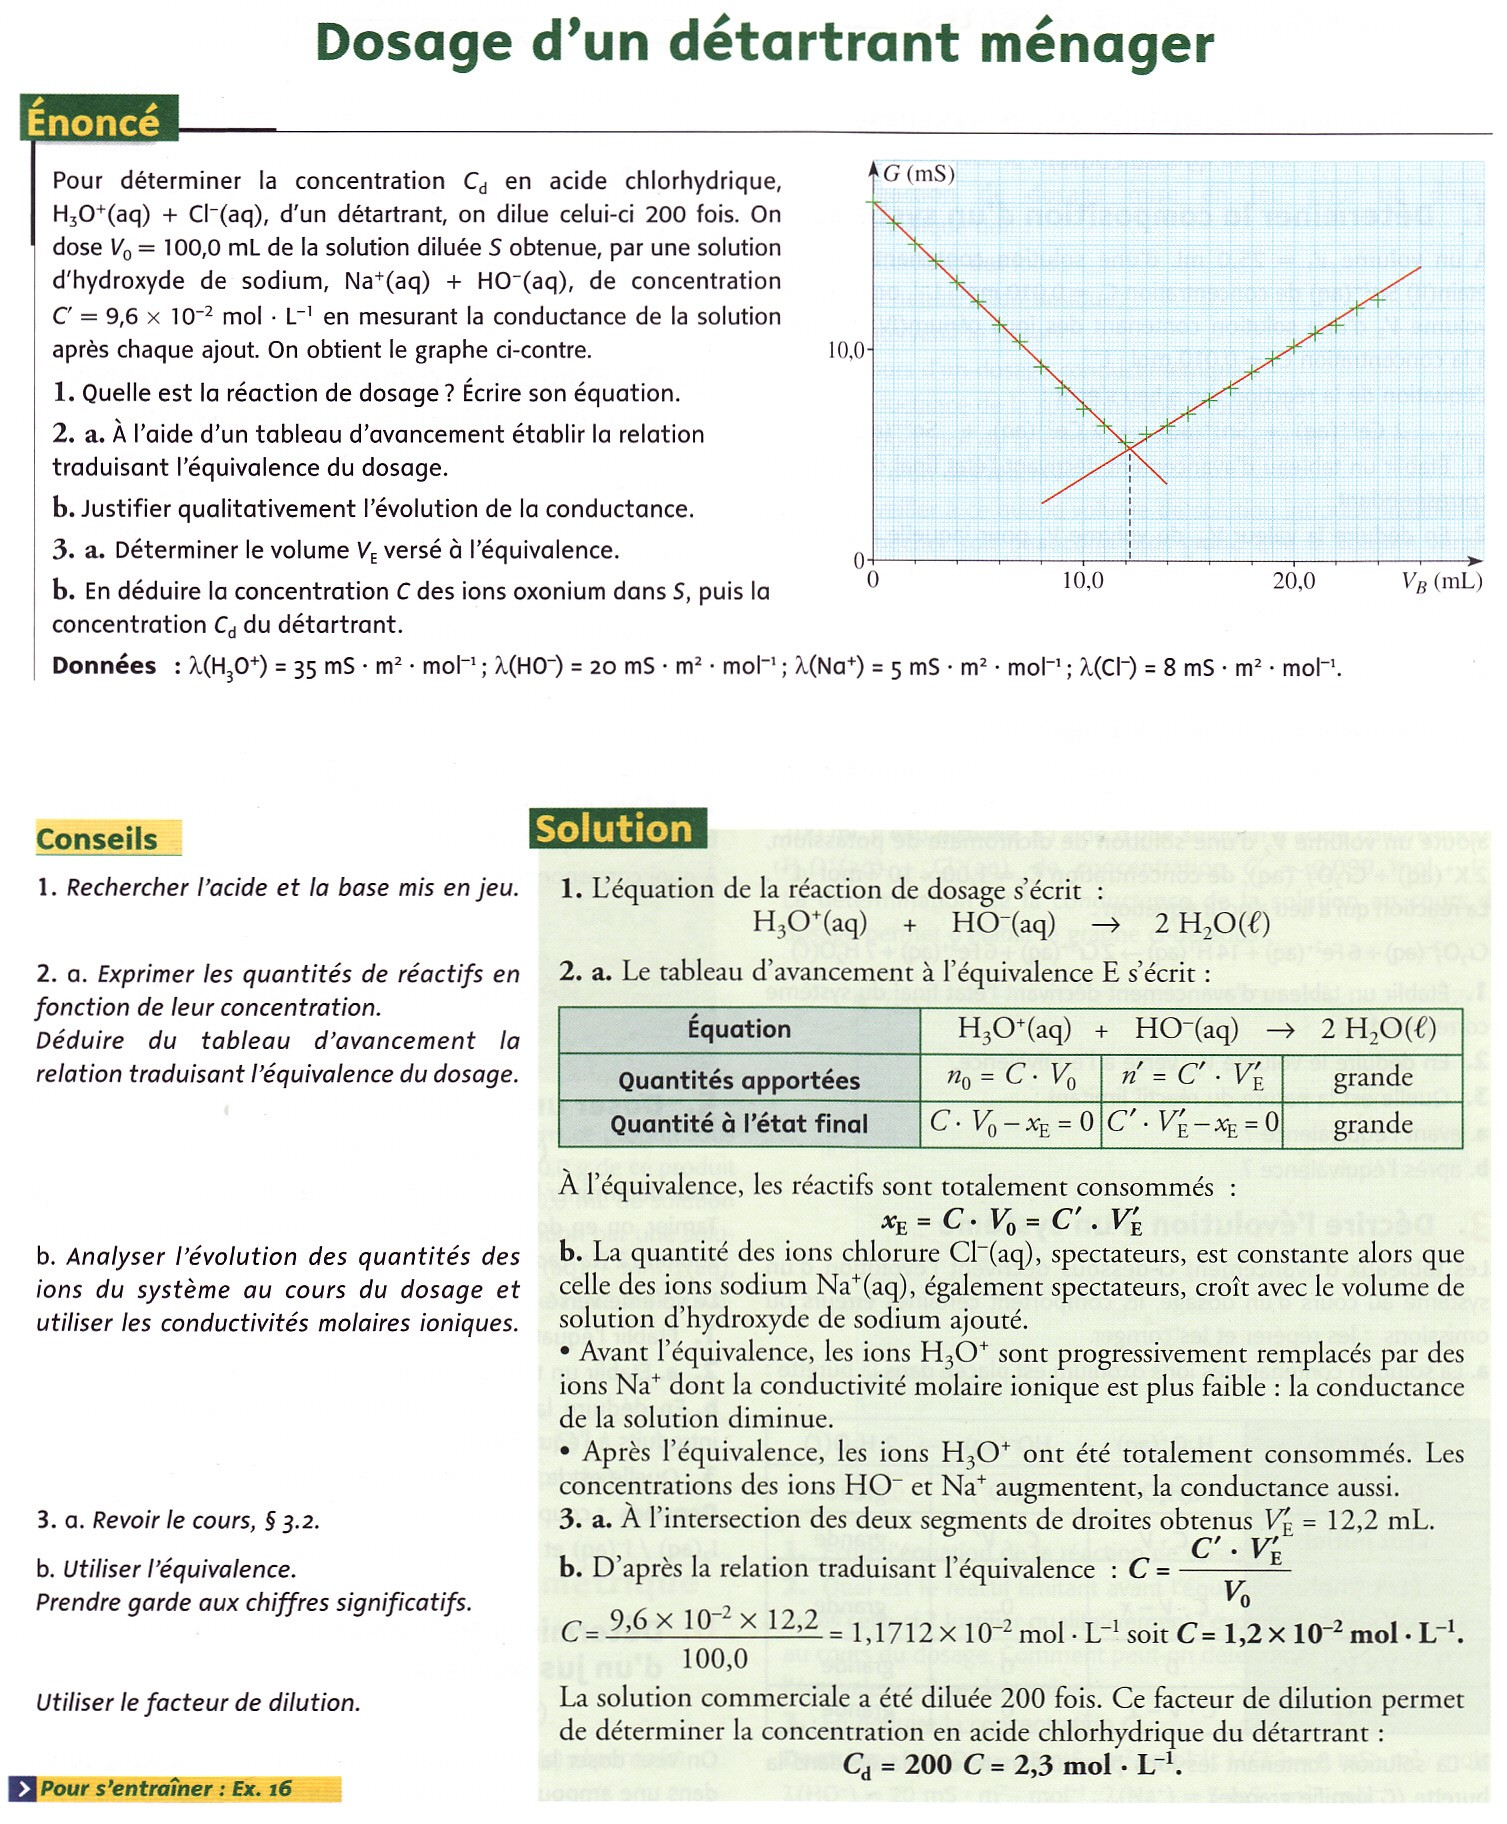
\includegraphics[width=\linewidth]{imgs/c1/xo4.jpg}
\end{figure} 
\begin{figure}[h]
    \centering
    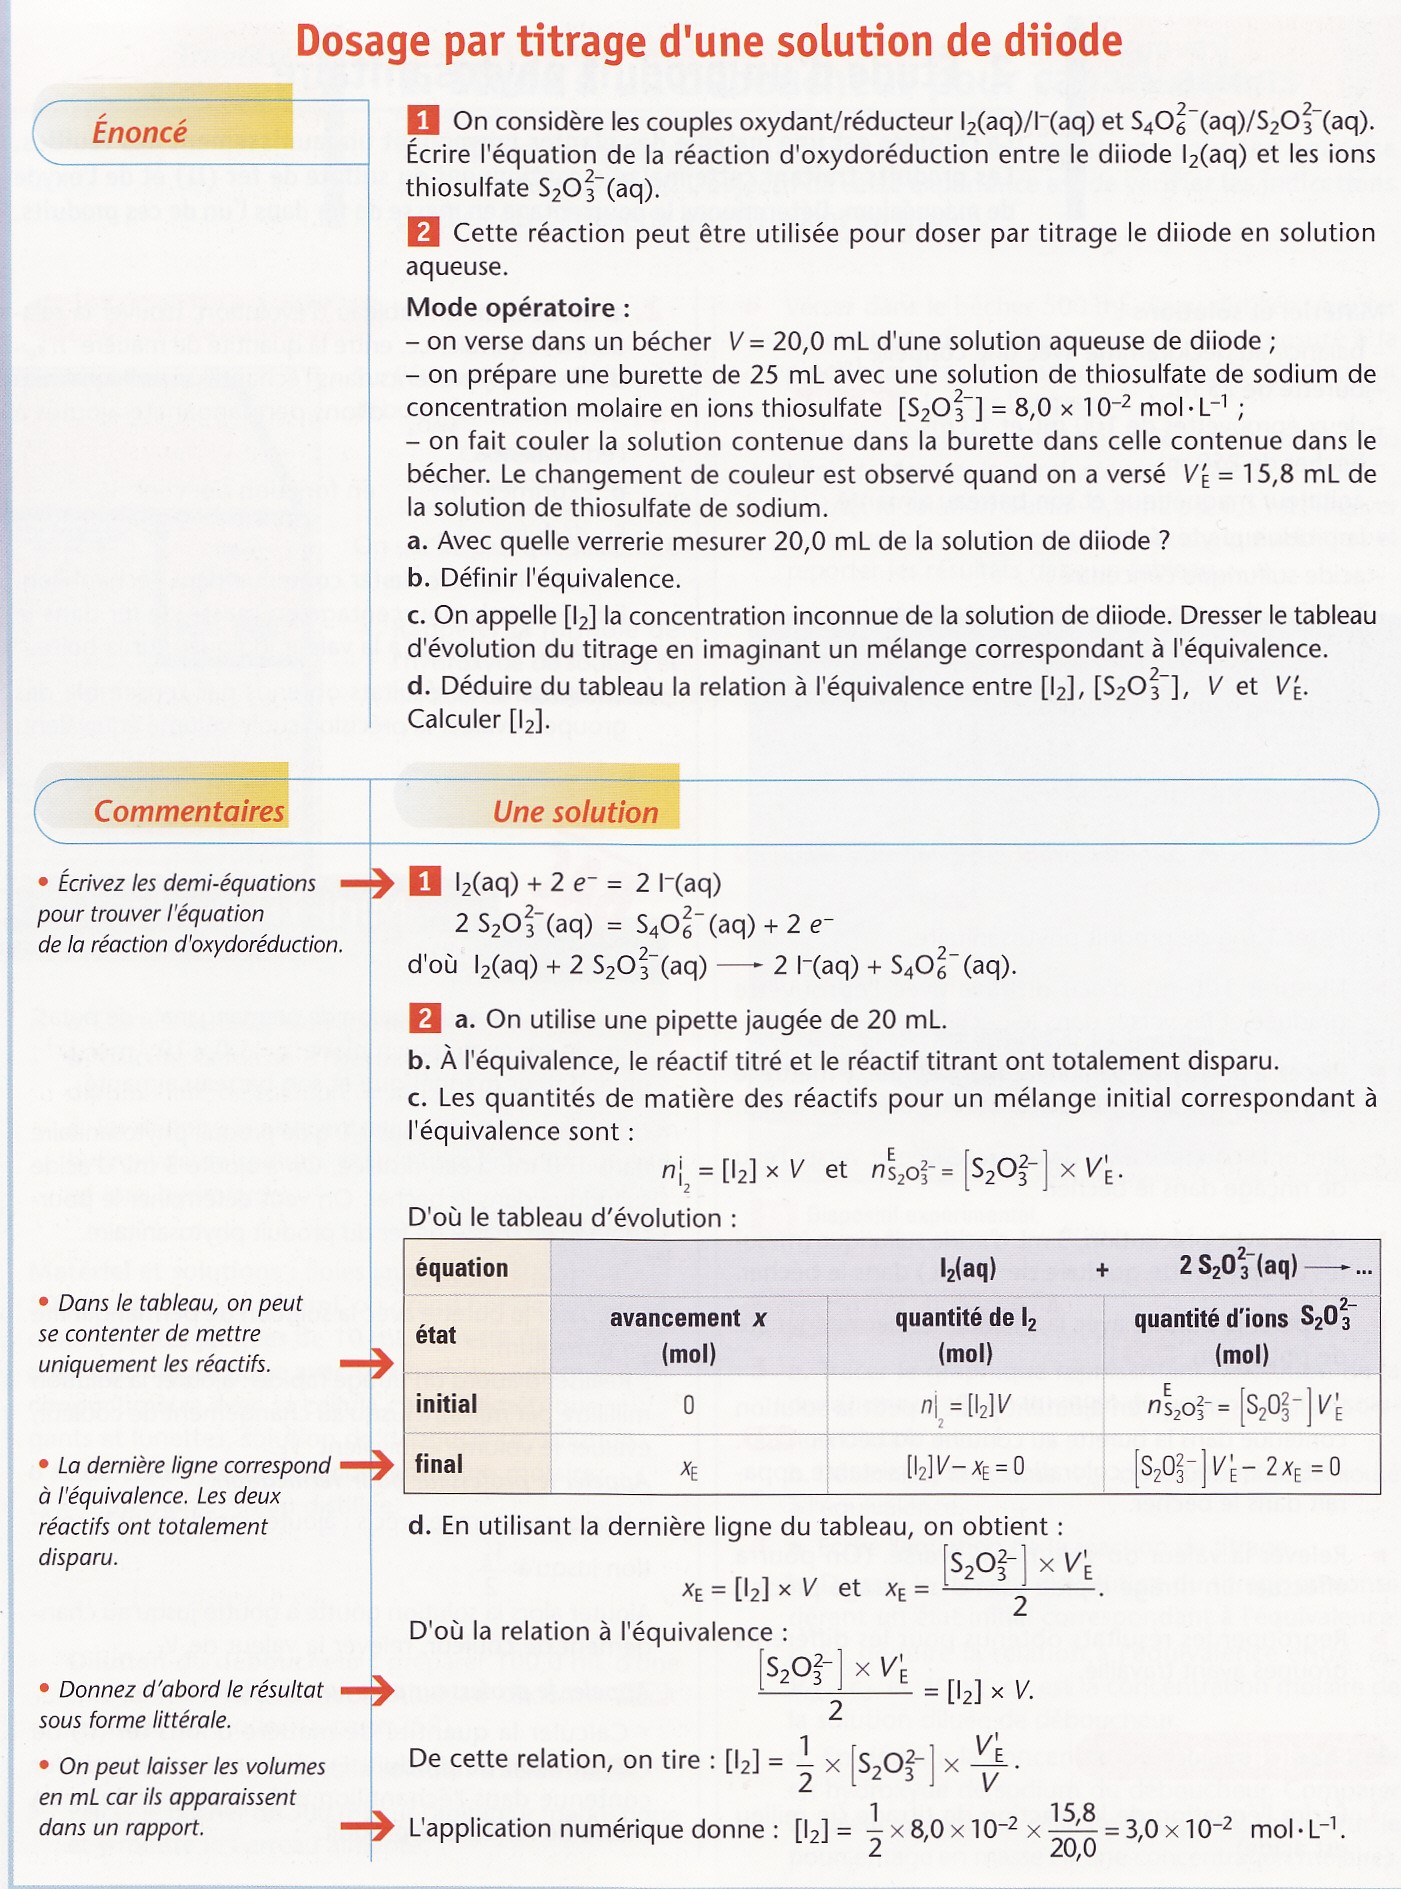
\includegraphics[width=\linewidth]{imgs/c1/xo5.jpg}
\end{figure} 
\begin{figure}[h]
    \centering
    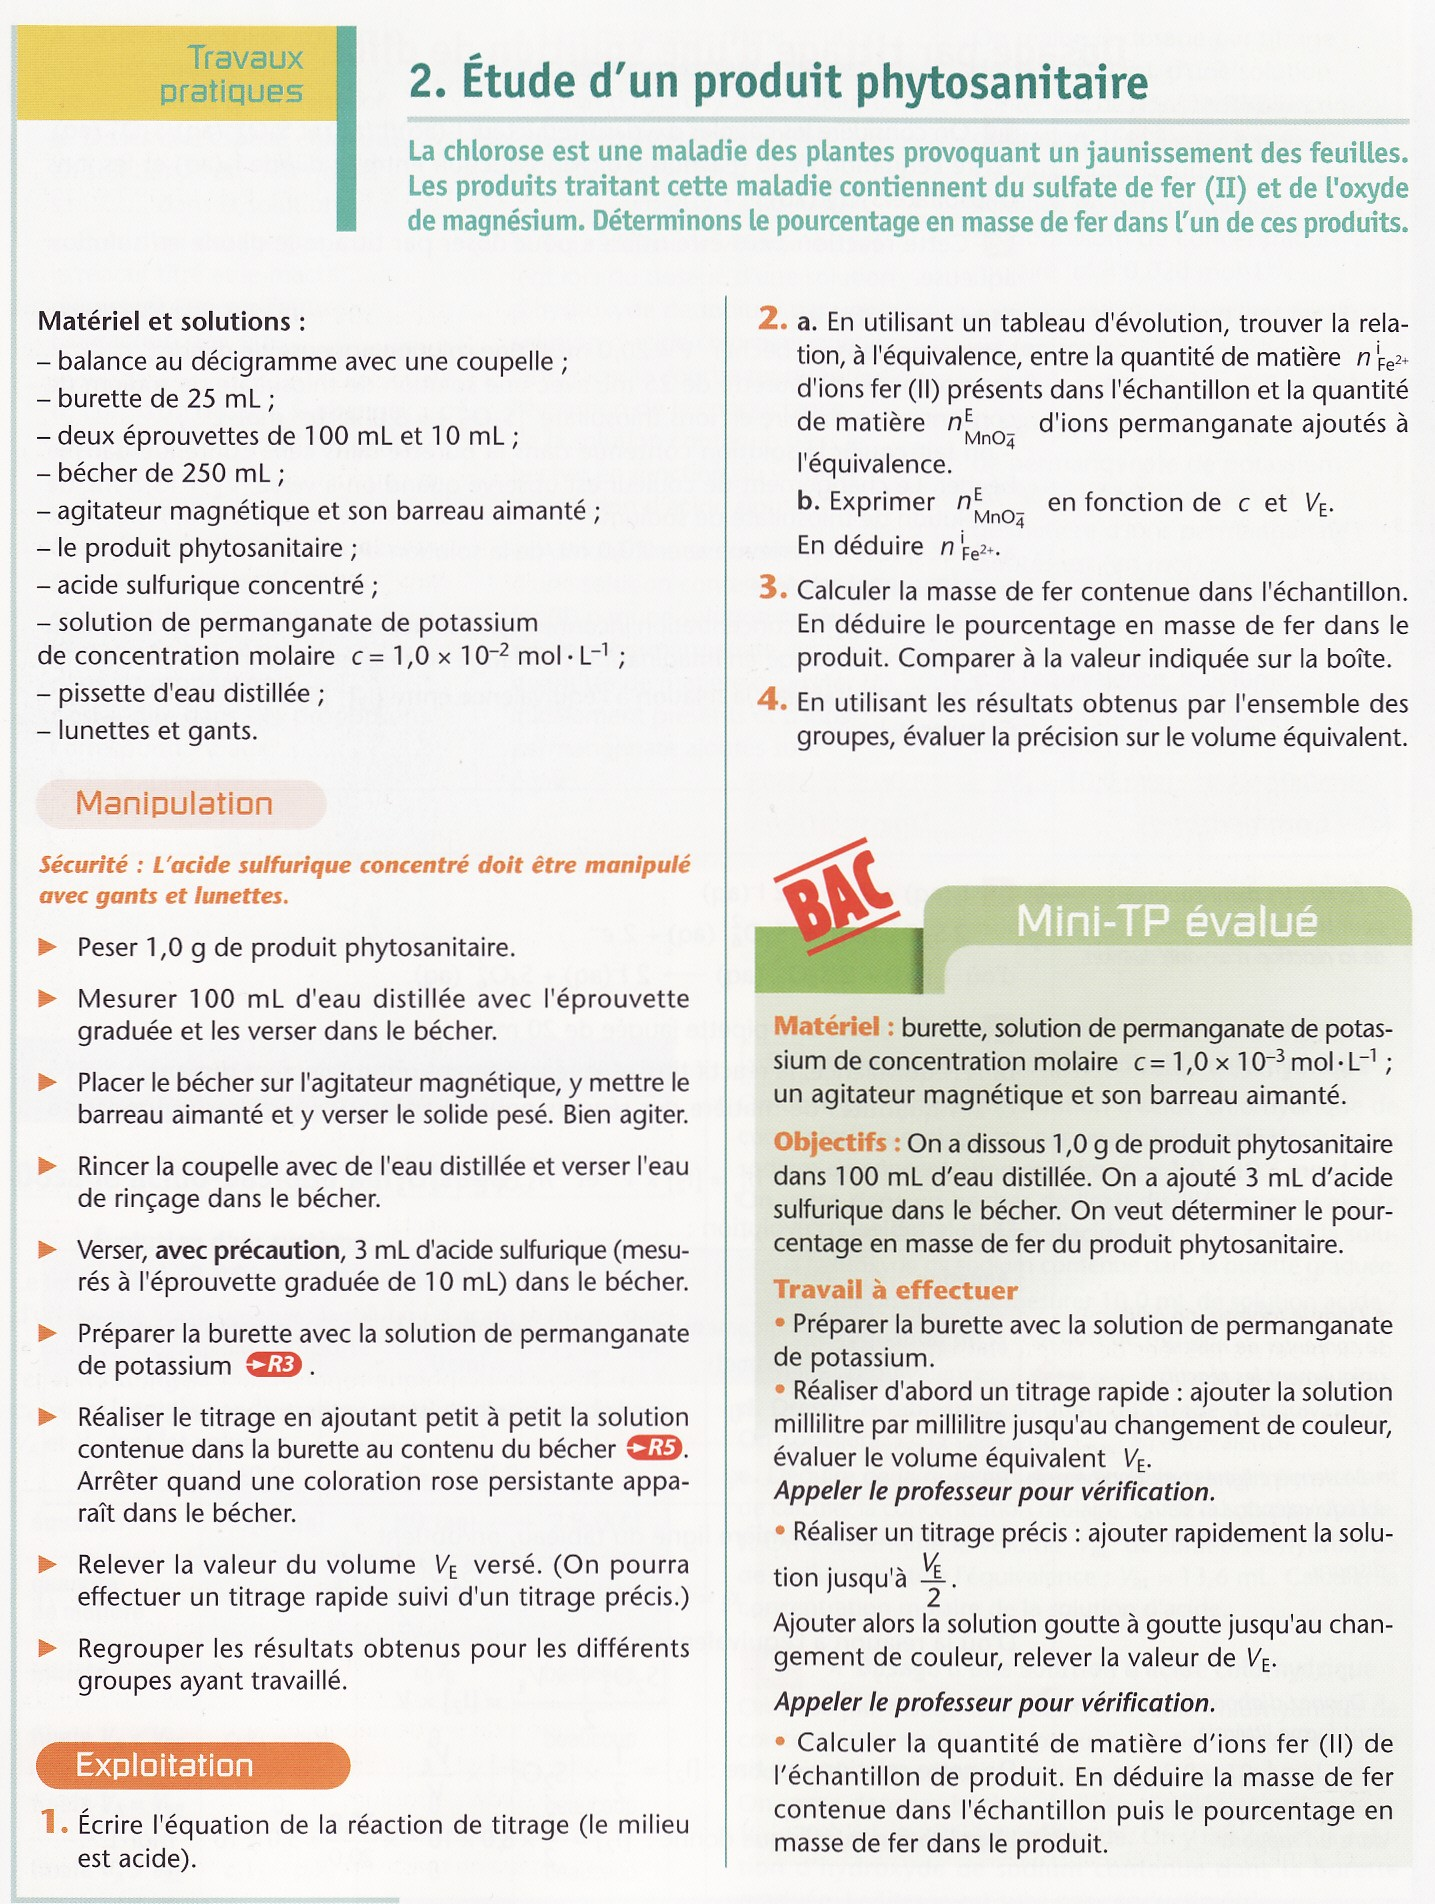
\includegraphics[width=\linewidth]{imgs/c1/xo6.jpg}
\end{figure} 

\begin{figure}[h]
    \centering
    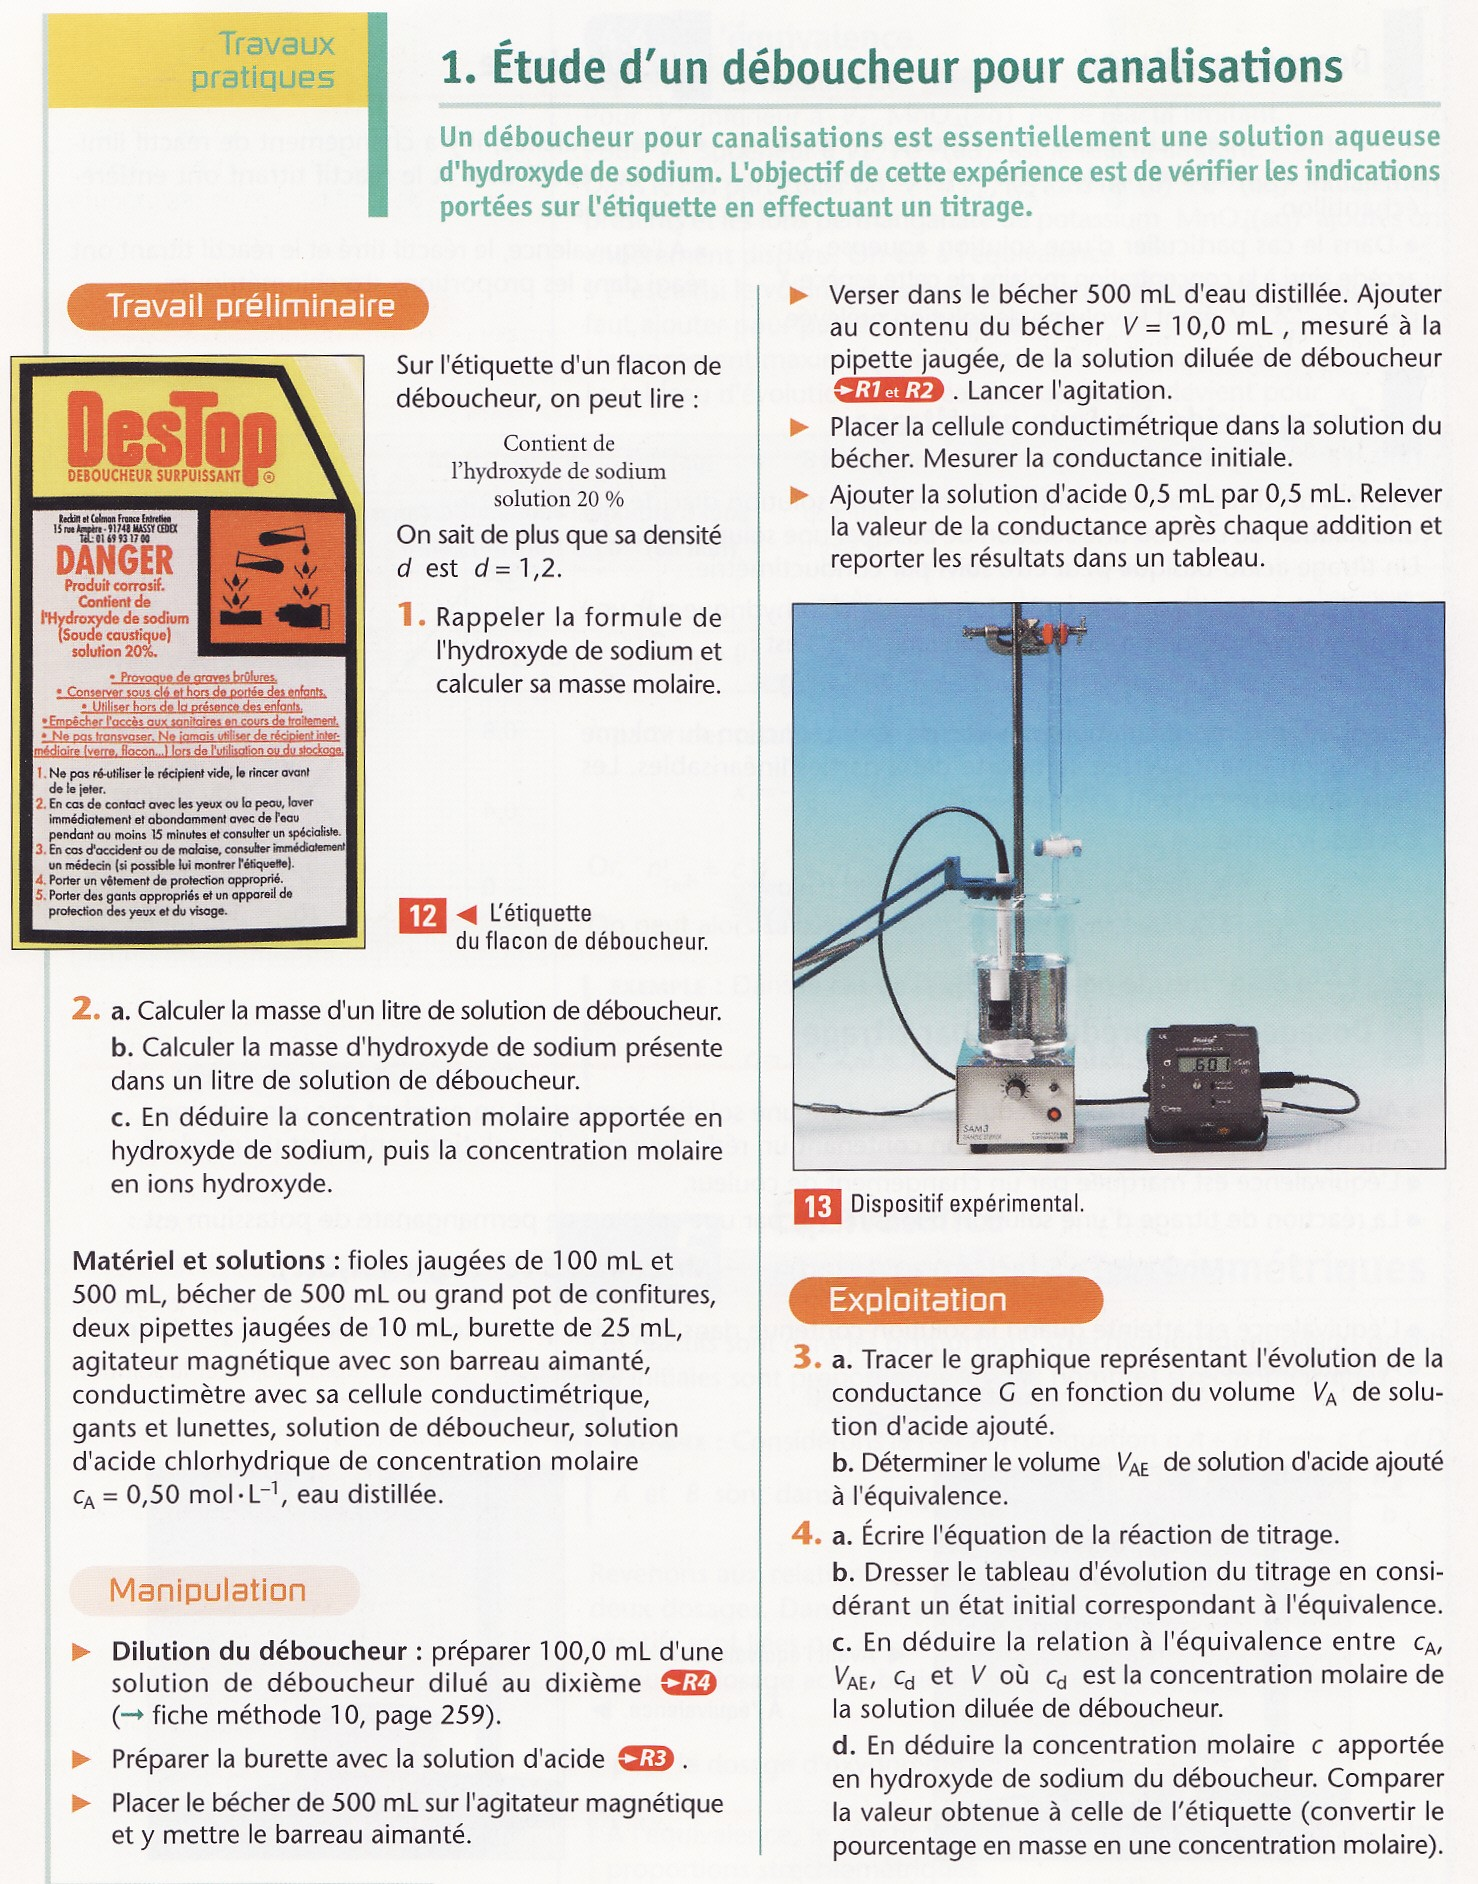
\includegraphics[width=\linewidth]{imgs/c1/xo7.jpg}
\end{figure} 

\end{document}